\documentclass[12pt, a4paper, oneside]{extarticle}

% --- Кодировка и локализация для XeLaTeX ---
\usepackage{fontspec}
\setmainfont{Liberation Serif} % Стандартный шрифт по ГОСТ.
\setmonofont{Liberation Mono}[Scale=MatchLowercase]
% Если компилируете на Linux без установленного Times New Roman,
% можно заменить на "Liberation Serif" или "PT Serif"

\usepackage[english,russian]{babel}

% --- Размеры полей (ГОСТ 7.32-2017: левое — 30 мм, правое — 10 мм, верхнее/нижнее — 20 мм) ---
\usepackage[
    left=30mm,
    right=10mm,
    top=20mm,
    bottom=20mm
]{geometry}

% --- Межстрочный интервал (ГОСТ требует полуторный) ---
\usepackage{setspace}
\onehalfspacing

% --- Абзацный отступ (ГОСТ: 1.25 см) ---
\usepackage{indentfirst} % Делает отступ в первом абзаце раздела
\setlength{\parindent}{1.25cm}

% --- Оформление заголовков (ГОСТ 7.32-2017) ---
\usepackage{titlesec}

% Команда для оформления структурных элементов (Введение, Заключение, Реферат и др.)
% По стандарту они не нумеруются, пишутся прописными буквами, центрируются и начинаются с новой страницы.
\newcommand{\goststruct}[1]{
    \clearpage
    \phantomsection
    \begin{center}
        \bfseries\MakeUppercase{#1}
    \end{center}
    \addcontentsline{toc}{section}{#1}
    \par\medskip
}

% Настройка нумеруемых разделов (Разделы основной части)
% Пишутся прописными (заглавными) буквами с абзацного отступа.
\titleformat{\section}
  {\normalfont\bfseries}
  {\thesection\quad}
  {0pt}
  {\MakeUppercase}

% Подразделы пишутся строчными буквами (кроме первой прописной) с абзацного отступа.
\titleformat{\subsection}
  {\normalfont\bfseries}
  {\thesubsection\quad}
  {0pt}
  {}

\titleformat{\subsubsection}
  {\normalfont\bfseries}
  {\thesubsubsection\quad}
  {0pt}
  {}

% Настройка интервалов до и после заголовков (в соответствии с абзацным отступом)
\titlespacing*{\section}{\parindent}{12pt}{6pt}
\titlespacing*{\subsection}{\parindent}{12pt}{6pt}
\titlespacing*{\subsubsection}{\parindent}{12pt}{6pt}

% --- Настройка содержания (Оглавления) ---
\usepackage{tocloft}
\renewcommand{\cftsecleader}{\cftdotfill{\cftdotsep}} % Точки для разделов в содержании
\addto\captionsrussian{\renewcommand{\contentsname}{СОДЕРЖАНИЕ}} % Заголовок прописью
\renewcommand{\cfttoctitlefont}{\hfill\bfseries\normalsize}  % Размер слова СОДЕРЖАНИЕ
\renewcommand{\cftaftertoctitle}{\hfill}

% Переименование списка литературы по ГОСТ
\addto\captionsrussian{\renewcommand{\refname}{СПИСОК ИСПОЛЬЗОВАННЫХ ИСТОЧНИКОВ}}

% --- Оформление подписей к рисункам и таблицам ---
\usepackage{caption}
\DeclareCaptionLabelSeparator{emdash}{~--- } % Разделитель — длинное тире

% Рисунки: подпись снизу, по центру, без абзацного отступа (например: Рисунок 1 — Название)
\captionsetup[figure]{
    name=Рисунок,
    labelsep=emdash,
    justification=centering,
    singlelinecheck=false,
    position=bottom,
    skip=6pt
}

% Таблицы: название сверху, слева, без абзацного отступа (например: Таблица 1 — Название)
\captionsetup[table]{
    name=Таблица,
    labelsep=emdash,
    justification=raggedright,
    singlelinecheck=false,
    position=top,
    skip=6pt
}

% --- Нумерация страниц (ГОСТ: внизу по центру, арабскими цифрами, без точки) ---
% На титульном листе номер не ставится, но он входит в общую нумерацию.
\usepackage{fancyhdr}
\pagestyle{fancy}
\fancyhf{}
\cfoot{\thepage}
\renewcommand{\headrulewidth}{0pt}
\renewcommand{\footrulewidth}{0pt}
\fancypagestyle{plain}{
    \fancyhf{}
    \cfoot{\thepage}
}

% --- Списки (ГОСТ требует дефисы вместо стандартных маркеров) ---
\usepackage{enumitem}
\setlist[itemize]{label=---, leftmargin=\parindent, itemsep=0pt, parsep=0pt}
\setlist[enumerate]{leftmargin=\parindent, itemsep=0pt, parsep=0pt}

% --- Дополнительные полезные пакеты ---
\usepackage{amsmath, amsfonts, amssymb} % Математика
\usepackage{graphicx}                  % Рисунки
\usepackage{booktabs}                  % Улучшенные таблицы
\usepackage{array}                     % Дополнительные настройки колонок
\usepackage[colorlinks=true, allcolors=black, pdfborder={0 0 0}]{hyperref} % Ссылки (для печати черные)




\usepackage{longtable}
\usepackage{array}
\usepackage{minted}
\usemintedstyle{default} % Доступно множество стилей: monokai, colorful, VS и др.
\usepackage{xcolor}




\begin{document}

% ==========================================
% ТИТУЛЬНЫЙ ЛИСТ
% ==========================================
\begin{titlepage}
    \thispagestyle{empty}
    \begin{center}
        \fontsize{12pt}{14pt}\selectfont
        \textbf{Министерство науки и высшего образования Российской Федерации} \\
        ФЕДЕРАЛЬНОЕ ГОСУДАРСТВЕННОЕ АВТОНОМНОЕ ОБРАЗОВАТЕЛЬНОЕ \\
        УЧРЕЖДЕНИЕ ВЫСШЕГО ОБРАЗОВАНИЯ \\
        \textbf{НАЦИОНАЛЬНЫЙ ИССЛЕДОВАТЕЛЬСКИЙ УНИВЕРСИТЕТ ИТМО} \\

        \vfill

        Факультет безопасности информационных технологий

        \vfill

        Дисциплина: \\
        «Алгоритмы и структуры данных»
        \vfill

        ОТЧЁТ ПО ЛАБОРАТОРНОЙ РАБОТЕ №5 \\
        «Решение уравнения Риккати с помощью General Projected Riccati Algorithm»

        \vfill

        \hfill
        \begin{flushright}
            Выполнил: \\
            Пахомов Владимир Юрьевич, студент группы N3250 \\

            \vspace{1.5cm}

            \begin{minipage}{0.2\textwidth}
                \begin{center}
                    \underline{\hspace{3cm}} \\
                    \fontsize{9pt}{11pt}\selectfont
                    (подпись)
                \end{center}
            \end{minipage}

            \vspace{1.5cm}

            Проверил: \\
            Ерофеев Сергей Анатольевич

            \vspace{1.5cm}

            \begin{minipage}{0.25\textwidth}
                \begin{center}
                    \underline{\hspace{4cm}} \\
                    \fontsize{9pt}{11pt}\selectfont
                    (отметка о выполнении)
                \end{center}
            \end{minipage}

            \vspace{1.5cm}

            \begin{minipage}{0.2\textwidth}
                \begin{center}
                    \underline{\hspace{3cm}} \\
                    \fontsize{9pt}{11pt}\selectfont
                    (подпись)
                \end{center}
            \end{minipage}
        \end{flushright}

        \vfill

        \fontsize{12pt}{14pt}\selectfont
        Санкт-Петербург \\
        2026
    \end{center}
\end{titlepage}

\newpage
% Начинаем нумерацию со 2-й страницы (титульный лист был первым, но без номера)
\setcounter{page}{2}

% ==========================================
% СОДЕРЖАНИЕ
% ==========================================
\clearpage
\tableofcontents

% ==========================================
% ВВЕДЕНИЕ
% ==========================================
\goststruct{Введение}
\textbf{Цель работы} --- изучение теоретических основ проекционных методов редукции моделей (Model Order Reduction) и практическая разработка программного комплекса для численного решения непрерывного алгебраического уравнения Риккати (CARE) на основе проекционного алгоритма (General Projected Riccati Algorithm).

Для достижения поставленной цели в рамках лабораторной работы решаются следующие задачи:
\begin{enumerate}
    \item Изучение и реализация метода собственных ортогональных компонент (POD — Proper Orthogonal Decomposition) на основе траектории (снимков состояния) сопряженной системы, интегрируемой численным методом Рунге-Кутты 4-го порядка.
    \item Реализация алгоритма проецирования исходной высокоразмерной системы $(A,B,C)$ на ортонормированный POD-базис для получения редуцированной системы меньшего порядка.
    \item Реализация итерационного метода Ньютона-Клейнмана для решения уравнения Риккати малой размерности.
    \item Разработка алгоритма решения общих (в том числе несимметричных) уравнений Ляпунова, возникающих на каждом шаге метода Ньютона, с использованием Кронекеровой векторизации и метода Гаусса с частичным выбором ведущего элемента.
    \item Проведение численных экспериментов на тестовых моделях различной структуры и оценка нормы невязки восстановленного решения в зависимости от размерности проекционного пространства ($l$).
\end{enumerate}

% ==========================================
% ОСНОВНАЯ ЧАСТЬ
% ==========================================
\clearpage
\section{Описание работы алгоритма и реализации программы}

Программный комплекс реализован на языке C в виде консольного приложения,
работающего со стандартными потоками ввода-вывода (\texttt{stdin}/\texttt{stdout}).

Рассматривается линейная непрерывная динамическая система вида:
\begin{align}
    \dot{x}(t) &= A\,x(t) + B\,u(t), \label{eq:state} \\
    y(t)       &= C\,x(t),            \label{eq:output}
\end{align}
где $x(t) \in \mathbb{R}^N$ --- вектор состояния, $u(t) \in \mathbb{R}^m$ ---
вектор управления, $y(t) \in \mathbb{R}^p$ --- вектор измеримых выходов.

Задача линейно-квадратичного регулятора (LQR) состоит в нахождении закона
управления $u(t) = -K x(t)$, минимизирующего квадратичный функционал:
\begin{equation}
    J = \int_0^{\infty} \bigl( x^T(t)\,Q\,x(t) + u^T(t)\,u(t) \bigr)\,dt,
    \label{eq:lqr}
\end{equation}
где штрафная матрица $Q = C^T C \geq 0$ задаётся через матрицу выходов.
Оптимальная матрица регулятора вычисляется как $K = B^T P$, где
$P \in \mathbb{R}^{N \times N}$ --- стабилизирующее решение \textit{непрерывного
алгебраического уравнения Риккати} (Continuous Algebraic Riccati Equation,
CARE):
\begin{equation}
    A^T P + P A - P B B^T P + C^T C = 0.
    \label{eq:riccati_equation}
\end{equation}

Матрицы системы имеют следующий физический смысл:
\begin{itemize}
    \item $A \in \mathbb{R}^{N \times N}$ --- \textbf{матрица динамики}: описывает
    свободную эволюцию системы~\eqref{eq:state} при $u \equiv 0$. Если все
    собственные значения $A$ имеют отрицательную вещественную часть, система
    устойчива без управления; наличие хотя бы одного собственного значения с
    положительной вещественной частью означает неустойчивость;

    \item $B \in \mathbb{R}^{N \times m}$ --- \textbf{матрица входов}: определяет,
    как управляющее воздействие $u(t)$ влияет на изменение каждой компоненты
    вектора состояния;

    \item $C \in \mathbb{R}^{p \times N}$ --- \textbf{матрица выходов}: задаёт,
    какие линейные комбинации компонент вектора состояния измеряются датчиками;

    \item $P \in \mathbb{R}^{N \times N}$ --- \textbf{искомая матрица решения}
    Риккати. В физически реализуемых системах $P$ симметрична ($P = P^T$) и
    положительно полуопределена ($P \geq 0$). Элемент $P_{ij}$ отражает
    «стоимость» совместного отклонения $i$-й и $j$-й компонент состояния ---
    насколько дорого (в смысле расхода управления) исправить данное отклонение
    оптимальным образом.
\end{itemize}

При $N$ большой размерности прямое решение уравнения~\eqref{eq:riccati_equation}
требует $O(N^3)$ операций и $O(N^2)$ памяти, что делает его неприемлемым для
задач большой размерности. Для преодоления этого ограничения применяется
\textit{General Projected Riccati Algorithm}: исходная система редуцируется на
подпространство малой размерности $l \ll N$, построенное методом POD, и
уравнение Риккати решается в этом подпространстве.

\subsection{Условия применимости алгоритма}

Для существования стабилизирующего решения $P \geq 0$
уравнения~\eqref{eq:riccati_equation} и корректной работы алгоритма необходимо
выполнение следующих условий.

\subsubsection{Стабилизируемость пары $(A,\,B)$}

Пара $(A, B)$ называется \textit{стабилизируемой}, если существует матрица $K$
такая, что замкнутая матрица $A - BK$ устойчива:
\begin{equation}
    \exists\;K\in\mathbb{R}^{m\times N}\colon\quad
    \operatorname{Re}\lambda_i(A - BK) < 0,\quad i = 1,\dots,N.
    \label{eq:stabilizability}
\end{equation}
Физически это означает, что все неустойчивые моды системы доступны для
управления через вход $u(t)$. Если какая-либо неустойчивая мода не зависит от
$B$, подавить её невозможно и стабилизирующего решения не существует.

Практически проверить стабилизируемость можно по критерию Хаутуса: пара
$(A, B)$ стабилизируема тогда и только тогда, когда
\begin{equation}
    \operatorname{rank}\begin{bmatrix} A - \lambda I & B \end{bmatrix} = N
    \quad\forall\,\lambda\in\mathbb{C},\quad\operatorname{Re}\lambda \geq 0.
    \label{eq:hautus_stab}
\end{equation}

\subsubsection{Обнаруживаемость пары $(C,\,A)$}

Пара $(C, A)$ называется \textit{обнаруживаемой}, если существует матрица $L$
такая, что матрица $A - LC$ устойчива:
\begin{equation}
    \exists\;L\in\mathbb{R}^{N\times p}\colon\quad
    \operatorname{Re}\lambda_i(A - LC) < 0,\quad i = 1,\dots,N.
    \label{eq:detectability}
\end{equation}
Физически это означает, что все неустойчивые моды системы отражаются в
измеримых выходах $y(t)$. Если неустойчивая мода не проявляется ни в одном
датчике, её нельзя обнаружить и, следовательно, стабилизировать по выходу.

Критерий Хаутуса для обнаруживаемости:
\begin{equation}
    \operatorname{rank}\begin{bmatrix} A - \lambda I \\ C \end{bmatrix} = N
    \quad\forall\,\lambda\in\mathbb{C},\quad\operatorname{Re}\lambda \geq 0.
    \label{eq:hautus_det}
\end{equation}

При выполнении условий~\eqref{eq:stabilizability} и~\eqref{eq:detectability}
стабилизирующее решение $P \geq 0$ уравнения~\eqref{eq:riccati_equation}
существует и единственно.

\subsubsection{Условие единственности решения уравнения Ляпунова}

На каждом шаге метода Ньютона--Клейнмана решается уравнение Ляпунова
относительно матрицы $A_{cl} = A_l - B_l B_l^T P_k$. Уравнение Ляпунова
$A_{cl}^T X + X A_{cl} = -F$ имеет единственное решение тогда и только тогда,
когда матрица $A_{cl}$ не имеет пар собственных значений $(\lambda_i, \lambda_j)$
таких, что $\lambda_i + \lambda_j = 0$. Достаточным условием является
устойчивость $A_{cl}$, которая обеспечивается при выполнении условий
стабилизируемости и обнаруживаемости уже начиная с нулевого приближения.

\subsubsection{Требования к параметрам POD-базиса}

Для получения содержательного проекционного подпространства необходимо:
\begin{enumerate}
    \item Конечное время $T_{final}$ должно быть достаточно большим, чтобы
    траектория сопряжённой системы $\dot{x} = A^T x$ охватила все существенные
    направления пространства состояний. Для устойчивых систем рекомендуется
    $T_{final} \gtrsim 5 / |\operatorname{Re}\lambda_{min}(A)|$, где
    $\lambda_{min}$ --- наименьшее по модулю собственное значение.

    \item Число шагов $steps$ должно обеспечивать точность метода Рунге--Кутты
    4-го порядка: рекомендуется $steps \geq 100$, чтобы шаг
    $\Delta t = T_{final}/steps$ был достаточно мал.

    \item Заданный ранг $r$ не должен превышать $N$. В программе это учтено
    автоматически: $r_{max} = \min(r, N)$.
\end{enumerate}

\subsection{Чтение входных данных и инициализация памяти}

При запуске программа выполняет последовательное считывание параметров модели и
матриц системы:
\begin{enumerate}
    \item Через стандартный поток ввода считывается заголовок, содержащий
    размерности исходной системы ($N, m, p$), целевой ранг проектора $r$,
    количество шагов интегрирования $steps$ и конечное время траектории
    $T_{final}$.

    \item Выполняется проверка корректности размерностей. Рабочий ранг
    проектора ограничивается физическим размером системы:
    $r_{max} = \min(r, N)$.

    \item С помощью функции \texttt{xcalloc} динамически выделяется память под
    одномерные массивы типа \texttt{double} для хранения матриц исходной
    системы:
    \begin{itemize}
        \item матрица динамики: $A \in \mathbb{R}^{N \times N}$;
        \item матрица входов: $B \in \mathbb{R}^{N \times m}$;
        \item матрица выходов: $C \in \mathbb{R}^{p \times N}$;
    \end{itemize}
    в строчном формате (row-major).

    \item Осуществляется построчное чтение элементов матриц $A$, $B$ и $C$.
\end{enumerate}

\subsection{Построение проектора методом POD (функция \texttt{build\_pod\_basis})}

Для формирования оптимального проекционного подпространства вызывается функция
\texttt{build\_pod\_basis}, выполняющая следующие действия:
\begin{enumerate}
    \item Выделяется память под траекторную матрицу снимков $Y$ размера
    $N \times S$, где общее число снимков $S = p \cdot (steps + 1)$.

    \item Запускается цикл по выходам системы $out = 0, \dots, p-1$. Для
    каждого выхода:
    \begin{itemize}
        \item В качестве начального вектора сопряжённого состояния
        $x(0) \in \mathbb{R}^N$ берётся строка с индексом $out$ матрицы
        выходов $C$, транспонированная в столбец:
        \begin{equation*}
            x(0) = C_{out,\,\cdot}^T.
        \end{equation*}
        \item На протяжении $steps$ шагов с шагом $\Delta t = T_{final}/steps$
        выполняется интегрирование сопряжённой системы:
        \begin{equation*}
            \dot{x}(t) = A^T x(t).
        \end{equation*}
        На каждом шаге новое состояние $x(t_s)$ вычисляется классическим
        методом Рунге--Кутты 4-го порядка (\texttt{rk4\_step\_AT}).
        \item Вектор состояния $x(t_s)$ на каждом шаге $s$ копируется в
        соответствующий столбец матрицы снимков $Y$.
    \end{itemize}

    \item Вычисляются элементы симметричной матрицы Грамиана
    $G \in \mathbb{R}^{S \times S}$ как скалярные произведения снимков,
    взвешенные по правилу трапеций:
    \begin{equation*}
        G_{a,b} = \Delta t \cdot w_a w_b \cdot \langle Y_{\cdot,a},\,
        Y_{\cdot,b}\rangle = \Delta t \cdot w_a w_b \sum_{i=1}^N Y_{i,a}\,Y_{i,b},
    \end{equation*}
    где весовые коэффициенты $w_a,\,w_b$ равны $0{,}5$ для начального и
    конечного снимков и $1{,}0$ для промежуточных.

    \item С помощью классического итерационного алгоритма вращений Якоби
    (\texttt{jacobi\_sym\_eigen}) находятся собственные значения $w$ и
    собственные векторы $U$ матрицы Грамиана $G$:
    \begin{equation*}
        G\,U_{\cdot,k} = \lambda_k\,U_{\cdot,k}, \quad k = 1, \dots, S.
    \end{equation*}

    \item Полученные пары $(\lambda_k,\,U_{\cdot,k})$ сортируются по убыванию
    собственных значений \\(\texttt{sort\_eigs\_desc}).

    \item Осуществляется фильтрация: в базис включаются только компоненты с
    $\lambda_k > 10^{-12}$. Рассчитывается эффективный ранг $r_{eff}$.

    \item Направления POD-мод формируются в матрице
    $V \in \mathbb{R}^{N \times r_{max}}$ по формуле:
    \begin{equation*}
        V_{i,k} = \frac{1}{\sqrt{\lambda_k}} \sum_{j=1}^S Y_{i,j}\,U_{j,k},
        \quad i = 1,\dots,N,\quad k = 1,\dots,r_{eff}.
    \end{equation*}

    \item Ввиду накопления численной погрешности при суммировании снимков,
    столбцы матрицы $V$ дополнительно ортонормируются процедурой
    Грама--Шмидта \\(\texttt{orthonormalize\_columns}).
\end{enumerate}

\subsection{Итерационный цикл редукции размерности}

После построения базиса определяется фактический диапазон исследования:\\
$r_{use} = \min(r,\,r_{eff})$. Программа запускает цикл по размерности
редуцированного подпространства $l = 1, \dots, r_{use}$. На каждом шаге $l$
выполняются следующие операции:
\begin{enumerate}
    \item Выделяется память под временный проектор $V_l$ размера $N \times l$,
    в который копируются первые $l$ столбцов из общего базиса $V$
    (\texttt{copy\_first\_columns}).

    \item Вызывается функция \texttt{project\_system}, вычисляющая
    спроецированные матрицы системы:
    \begin{align*}
        A_l &= V_l^T A V_l \in \mathbb{R}^{l \times l}, \\
        B_l &= V_l^T B    \in \mathbb{R}^{l \times m}, \\
        C_l &= C\,V_l     \in \mathbb{R}^{p \times l}.
    \end{align*}

    \item Инициализируется память под решение редуцированного уравнения
    Риккати $P_l \in \mathbb{R}^{l \times l}$, после чего вызывается функция
    \texttt{solve\_care\_newton} для решения:
    \begin{equation*}
        A_l^T P_l + P_l A_l - P_l B_l B_l^T P_l + C_l^T C_l = 0.
    \end{equation*}
\end{enumerate}

\subsubsection{Принцип решения уравнения Ляпунова методом Кронекеровой векторизации}

Уравнение Ляпунова в общем виде записывается следующим образом:
\begin{equation}
    A_{cl}^T X + X A_{cl} = -F,
    \label{eq:lyapunov}
\end{equation}
где $A_{cl} \in \mathbb{R}^{n \times n}$ --- заданная (не обязательно симметричная)
матрица, $F \in \mathbb{R}^{n \times n}$ --- известная правая часть, а
$X \in \mathbb{R}^{n \times n}$ --- искомая матрица. Несмотря на то что
уравнение~\eqref{eq:lyapunov} записано в матричном виде, его можно свести к
обычной системе линейных алгебраических уравнений (СЛАУ), применив операцию
векторизации.

\textbf{Операция векторизации.} Для матрицы $X \in \mathbb{R}^{n \times n}$
операция $\operatorname{vec}(X)$ формирует вектор размера $n^2$, последовательно
укладывая строки матрицы одна за другой:
\begin{equation*}
    \operatorname{vec}(X) =
    \begin{bmatrix}
        X_{1,1} & X_{1,2} & \cdots & X_{1,n} &
        X_{2,1} & \cdots & X_{n,n}
    \end{bmatrix}^T \in \mathbb{R}^{n^2}.
\end{equation*}

\textbf{Кронекерово произведение.} Для матриц $A \in \mathbb{R}^{p \times q}$ и
$B \in \mathbb{R}^{r \times s}$ кронекерово произведение определяется как блочная
матрица размера $pr \times qs$:
\begin{equation*}
    A \otimes B =
    \begin{bmatrix}
        A_{11} B & A_{12} B & \cdots & A_{1q} B \\
        A_{21} B & A_{22} B & \cdots & A_{2q} B \\
        \vdots   & \vdots   & \ddots & \vdots   \\
        A_{p1} B & A_{p2} B & \cdots & A_{pq} B
    \end{bmatrix}.
\end{equation*}

\textbf{Ключевое тождество.} Для произведения трёх матриц выполняется:
\begin{equation}
    \operatorname{vec}(AXB) = (B^T \otimes A)\,\operatorname{vec}(X).
    \label{eq:kron_identity}
\end{equation}

\textbf{Сведение уравнения Ляпунова к СЛАУ.} Применим
тождество~\eqref{eq:kron_identity} к каждому слагаемому
уравнения~\eqref{eq:lyapunov}. Запишем левую часть, используя единичную матрицу
$I_n$:
\begin{align*}
    \operatorname{vec}(A_{cl}^T X)
        &= \operatorname{vec}(A_{cl}^T \cdot X \cdot I_n)
         = (I_n \otimes A_{cl}^T)\,\operatorname{vec}(X), \\
    \operatorname{vec}(X A_{cl})
        &= \operatorname{vec}(I_n \cdot X \cdot A_{cl})
         = (A_{cl}^T \otimes I_n)\,\operatorname{vec}(X).
\end{align*}
Складывая оба выражения, получаем СЛАУ размера $n^2 \times n^2$:
\begin{equation}
    \underbrace{\bigl(I_n \otimes A_{cl}^T + A_{cl}^T \otimes I_n\bigr)}_{\mathcal{K}}
    \operatorname{vec}(X)
    = \operatorname{vec}(-F),
    \label{eq:kron_system}
\end{equation}
где матрица $\mathcal{K} \in \mathbb{R}^{n^2 \times n^2}$ называется
\textit{матрицей Кронекеровой суммы}.

\textbf{Заполнение матрицы $\mathcal{K}$ в строчно-мажорной адресации.}
В реализации на языке C матрицы хранятся в строчном формате (row-major), поэтому
элемент $X_{i,j}$ соответствует позиции $\operatorname{vec}(X)[i \cdot n + j]$.
Раскрывая определение Кронекеровой суммы поэлементно, для каждой строки
$\text{row} = i \cdot n + j$ матрицы $\mathcal{K}$ ненулевые вклады дают два
набора элементов:
\begin{align*}
    \mathcal{K}_{\,(i \cdot n + j),\,(k \cdot n + j)}
        &\mathrel{+}= (A_{cl})_{k,\,i}, \quad k = 0,\dots,n-1
        \quad\text{(вклад от слагаемого $I_n \otimes A_{cl}^T$),} \\
    \mathcal{K}_{\,(i \cdot n + j),\,(i \cdot n + k)}
        &\mathrel{+}= (A_{cl})_{k,\,j}, \quad k = 0,\dots,n-1
        \quad\text{(вклад от слагаемого $A_{cl}^T \otimes I_n$).}
\end{align*}
В каждой строке ненулевых элементов не более $2n$, что соответствует структуре
уравнения Ляпунова.

\textbf{Решение СЛАУ и извлечение результата.} Система~\eqref{eq:kron_system}
решается методом Гаусса с частичным выбором ведущего элемента по столбцу
(\texttt{gauss\_solve}), после чего решение $\operatorname{vec}(X)$ переформируется
обратно в матрицу $X \in \mathbb{R}^{n \times n}$.

\textbf{Вычислительная сложность.} Построение матрицы $\mathcal{K}$ требует
$O(n^3)$ операций. Решение СЛАУ методом Гаусса для матрицы размера
$n^2 \times n^2$ требует $O(n^6)$ операций. Именно поэтому данный подход
применяется только к \textit{редуцированным} уравнениям малой размерности
$l \ll N$: при $l = 5$ система имеет размер $25 \times 25$, при $l = 10$ ---
$100 \times 100$, что вычислительно приемлемо. Для исходной системы размера
$N \times N$ прямое применение данного метода потребовало бы решения СЛАУ
размера $N^2 \times N^2$, что и мотивирует использование проекционной редукции.

\textbf{Пример для скалярного случая.} При $n = 1$ уравнение Ляпунова
$A_{cl}^T X + X A_{cl} = -F$ принимает вид $2 A_{cl} X = -F$, откуда
$X = -F / (2 A_{cl})$. Матрица Кронекеровой суммы вырождается в скаляр
$\mathcal{K} = 2 A_{cl}$, что полностью согласуется с общей формулой.

\textbf{Условие существования решения.} Система~\eqref{eq:kron_system} имеет
единственное решение тогда и только тогда, когда матрица $\mathcal{K}$
невырождена, то есть когда у $A_{cl}$ нет пар собственных значений
$(\lambda_i, \lambda_j)$ таких, что $\lambda_i + \lambda_j = 0$. На практике
это условие обеспечивается устойчивостью $A_{cl}$ (все
$\operatorname{Re}\lambda_i < 0$), которая гарантируется методом
Ньютона--Клейнмана при выполнении условий стабилизируемости и обнаруживаемости
исходной системы.

\subsection{Метод Ньютона--Клейнмана и решатель уравнений Ляпунова}

Внутри функции \texttt{solve\_care\_newton} выполняется итерационный поиск
решения $P_l$:
\begin{enumerate}
    \item Находится начальное приближение $P_0$ путём решения уравнения
    Ляпунова:
    \begin{equation*}
        A_l^T P_0 + P_0 A_l = -C_l^T C_l
    \end{equation*}
    (функция \texttt{solve\_lyapunov}) и последующей принудительной
    симметризации (\texttt{symmetrize}).

    \item Запускается цикл итераций метода Ньютона--Клейнмана (до
    \texttt{MAX\_NEWTON\_ITERS} шагов). На каждом шаге $k$ вычисляется новое
    приближение:
    \begin{equation*}
        P_{k+1} = P_k + \Delta_k,
    \end{equation*}
    где поправка $\Delta_k \in \mathbb{R}^{l \times l}$ находится из уравнения
    Ляпунова:
    \begin{equation*}
        A_{cl}^T \Delta_k + \Delta_k A_{cl} = -F(P_k),
    \end{equation*}
    причём:
    \begin{align*}
        A_{cl}  &= A_l - B_l B_l^T P_k \in \mathbb{R}^{l \times l}
                   \quad\text{--- замкнутая матрица системы,}\\
        F(P_k)  &= A_l^T P_k + P_k A_l - P_k B_l B_l^T P_k + C_l^T C_l
                   \in \mathbb{R}^{l \times l}
                   \quad\text{--- невязка на итерации }k.
    \end{align*}
    Итерационный процесс прерывается, если $\|F(P_k)\|_F < \texttt{tol} =
    10^{-10}$.

    \item Для решения уравнения Ляпунова относительно несимметричной матрицы
    $A_{cl}$ в функции \texttt{solve\_lyapunov} строится СЛАУ Кронекеровой
    суммы размера $l^2 \times l^2$:
    \begin{equation*}
        \mathcal{K} \cdot \operatorname{vec}(\Delta_k)
        = \operatorname{vec}(-F(P_k)),
    \end{equation*}
    где:
    \begin{equation*}
        \mathcal{K} = I_l \otimes A_{cl}^T + A_{cl}^T \otimes I_l
        \in \mathbb{R}^{l^2 \times l^2}.
    \end{equation*}
    С учётом строчно-мажорной адресации в C-коде коэффициенты матрицы
    $\mathcal{K}$ инкрементируются по правилу:
    \begin{align*}
        \mathcal{K}_{(il+j),\,(hl+j)} &\leftarrow
        \mathcal{K}_{(il+j),\,(hl+j)} + (A_{cl})_{h,i}, \\
        \mathcal{K}_{(il+j),\,(il+h)} &\leftarrow
        \mathcal{K}_{(il+j),\,(il+h)} + (A_{cl})_{h,j},
    \end{align*}
    для всех $i,j,h = 0,\dots,l-1$.

    \item Полученная СЛАУ решается методом Гаусса с частичным выбором
    ведущего элемента по столбцу (\texttt{gauss\_solve}).

    \item Решение обновляется и симметризуется на каждом шаге.
\end{enumerate}

\subsection{Восстановление решения и оценка полной невязки}

После сходимости редуцированного решения $P_l$ программа оценивает его качество
относительно исходной системы $N \times N$:
\begin{enumerate}
    \item Вызывается функция \texttt{projected\_full\_residual}, которая
    восстанавливает полноразмерное приближение:
    \begin{equation*}
        P^{(N)} = V_l P_l V_l^T \in \mathbb{R}^{N \times N}.
    \end{equation*}

    \item Вычисляется матрица невязки исходного уравнения Риккати:
    \begin{equation*}
        R\!\left(P^{(N)}\right)
        = A^T P^{(N)} + P^{(N)} A - P^{(N)} B B^T P^{(N)} + C^T C
        \in \mathbb{R}^{N \times N}.
    \end{equation*}

    \item Рассчитывается норма Фробениуса невязки $\|R(P^{(N)})\|_F$.

    \item На экран выводится строка отчёта: текущая размерность $l$, число
    итераций Ньютона и норма невязки.

    \item Освобождается локальная динамическая память текущего шага $l$.
\end{enumerate}

После прохода по всем $l = 1,\dots,r_{use}$ программа освобождает память,
занятую матрицами $A,B,C$ и базисом $V$, и завершает работу.

\subsection{Физический смысл матриц и примеры применения}

\subsubsection{Пример 1. Стабилизация обратного маятника}

Задача состоит в удержании неустойчивого маятника в вертикальном положении за
счёт движения тележки. Линеаризованная модель вблизи положения равновесия имеет
вид~\eqref{eq:state}--\eqref{eq:output} с вектором состояния
$x = [s,\;\theta,\;\dot{s},\;\dot{\theta}]^T$, где $s$ --- смещение тележки,
$\theta$ --- угол отклонения маятника от вертикали.

Для типичных параметров ($M = 1{,}0$ кг, $m_p = 0{,}1$ кг, $L = 0{,}5$ м,
$g = 9{,}81$ м/с$^2$, $d = 0{,}1$) матрицы системы принимают вид:
\[
A \approx
\begin{bmatrix}
0      & 0       & 1      & 0    \\
0      & 0       & 0      & 1    \\
0      & -0{,}981 & -0{,}1 & 0    \\
0      & 21{,}582 &  0{,}2 & 0
\end{bmatrix},\quad
B =
\begin{bmatrix} 0 \\ 0 \\ 1{,}0 \\ -2{,}0 \end{bmatrix},\quad
C =
\begin{bmatrix} 1 & 0 & 0 & 0 \\ 0 & 1 & 0 & 0 \end{bmatrix}.
\]

Положительный элемент $A_{42} = 21{,}582$ означает, что угловое ускорение
маятника растёт при любом ненулевом угле --- система неустойчива без управления.
Матрица $B$ показывает, что управляющая сила воздействует только на ускорения
$\ddot{s}$ и $\ddot{\theta}$. Матрица $C$ означает, что датчики измеряют только
$s$ (энкодер) и $\theta$ (гироскоп), но не скорости.

Решение уравнения Риккати $P \in \mathbb{R}^{4 \times 4}$ даёт матрицу
регулятора $K = B^T P \in \mathbb{R}^{1 \times 4}$, при которой все собственные
значения замкнутой матрицы $A - BK$ приобретают отрицательную вещественную
часть, то есть система стабилизируется.

\subsubsection{Пример 2. Управление температурой в трёхзонной промышленной печи}

Задача --- поддерживать заданный профиль температур в трёх зонах печи при
минимальном расходе энергии. Вектор состояния $x = [T_1, T_2, T_3]^T$ содержит
отклонения температур от заданного значения.

Для коэффициентов теплообмена $k_{12} = k_{21} = 0{,}5$,
$k_{23} = k_{32} = 0{,}3$ и рассеяния $\alpha = 0{,}1$ матрицы принимают вид:
\[
A =
\begin{bmatrix}
-0{,}6 &  0{,}5 & 0      \\
 0{,}5 & -0{,}9 & 0{,}3  \\
 0     &  0{,}3 & -0{,}4
\end{bmatrix},\quad
B =
\begin{bmatrix} 1{,}0 & 0 \\ 0 & 0 \\ 0 & 1{,}0 \end{bmatrix},\quad
C = I_3.
\]

Все диагональные элементы матрицы $A$ по модулю превышают сумму остальных
элементов в своей строке, поэтому все собственные значения $A$ отрицательны ---
без нагревателей все зоны постепенно охлаждаются до температуры окружающей
среды. Нулевая строка в $B$ отражает факт, что 2-я зона не имеет собственного
нагревателя и нагревается только через теплообмен с соседями. Единичная матрица
$C = I_3$ означает, что термопары установлены во всех трёх зонах.

Решение уравнения Риккати даёт матрицу $K = B^T P \in \mathbb{R}^{2 \times 3}$
--- оптимальные коэффициенты обратной связи для двух нагревателей в зависимости
от отклонений температур во всех трёх зонах.

\subsection{Пример численного решения и проверка условий применимости}

Рассмотрим простейшую одномерную неустойчивую систему ($N = 1$, $m = 1$,
$p = 1$):
\begin{equation*}
    \dot{x}(t) = a\,x(t) + b\,u(t),\quad y(t) = c\,x(t),
\end{equation*}
с параметрами $A = [2]$, $B = [1]$, $C = [\sqrt{5}]$.

\textbf{Проверка условий применимости.}
\begin{itemize}
    \item \textit{Стабилизируемость~\eqref{eq:hautus_stab}:} для единственного
    собственного значения $\lambda = 2 > 0$ матрица
    $[A - \lambda I\;\;B] = [2 - 2\;\;1] = [0\;\;1]$ имеет ранг 1~$= N$.
    Условие выполнено: неустойчивая мода управляема.

    \item \textit{Обнаруживаемость~\eqref{eq:hautus_det}:} матрица
    $\begin{bmatrix}A - \lambda I\\ C\end{bmatrix}
    = \begin{bmatrix}0\\ \sqrt{5}\end{bmatrix}$ имеет ранг 1~$= N$.
    Условие выполнено: неустойчивая мода наблюдаема.
\end{itemize}

Таким образом, стабилизирующее решение $P > 0$ существует и единственно.

\textbf{Аналитическое решение.} Подставляя параметры
в~\eqref{eq:riccati_equation}:
\begin{equation*}
    2P + P \cdot 2 - P \cdot 1 \cdot 1 \cdot P + 5 = 0
    \implies P^2 - 4P - 5 = 0.
\end{equation*}
Корни: $P_{1,2} = \dfrac{4 \pm \sqrt{36}}{2}$, откуда $P_1 = 5$, $P_2 = -1$.
Поскольку требуется $P > 0$, единственным физически реализуемым решением
является:
\begin{equation*}
    P = 5.
\end{equation*}

\textbf{Синтез регулятора и проверка устойчивости.} Матрица регулятора:
$K = B^T P = 1 \cdot 5 = 5$, закон управления: $u(t) = -5\,x(t)$. Замкнутая
матрица системы:
\begin{equation*}
    A_{cl} = A - BK = 2 - 1 \cdot 5 = -3.
\end{equation*}
Так как $A_{cl} = -3 < 0$, замкнутая система асимптотически устойчива:
\begin{equation*}
    x(t) = x(0)\,e^{-3t} \;\to\; 0 \quad\text{при}\quad t \to \infty.
\end{equation*}
Таким образом, оптимальное управление $u(t) = -5\,x(t)$ не только стабилизирует
изначально неустойчивую систему ($A = 2 > 0$), но и минимизирует функционал
качества~\eqref{eq:lqr}.








\clearpage
\section{Описание используемых переменных}

Ниже представлена таблица с описанием использованных переменных.

\begin{longtable}{| >{\raggedright\arraybackslash}p{2.3cm}| >{\raggedright\arraybackslash}p{2.2cm}| >{\raggedright\arraybackslash}p{3.5cm}| >{\raggedright\arraybackslash}p{6.5cm}| }
\caption{Спецификация переменных программы} \label{tab:variables_spec} \\
\hline
\textbf{Название} & \textbf{Тип} & \textbf{Границы типа} & \textbf{Назначение} \\
\hline
\endfirsthead
\hline
\textbf{Название} & \textbf{Тип} & \textbf{Границы типа} & \textbf{Назначение} \\
\hline
\endhead
\hline
\endfoot
\hline
\endlastfoot

\multicolumn{4}{|l|}{\textit{Параметры и структуры исходной динамической системы}} \\
\hline
\texttt{N} & \texttt{int} & от 1 до $2^{31}-1$ & Размерность вектора состояния исходной системы. \\
\hline
\texttt{m} & \texttt{int} & от 1 до $2^{31}-1$ & Количество входов (размерность управления). \\
\hline
\texttt{p} & \texttt{int} & от 1 до $2^{31}-1$ & Количество выходов (размерность измерения). \\
\hline
\texttt{r} & \texttt{int} & от 1 до $2^{31}-1$ & Заданный максимальный ранг проекционного подпространства. \\
\hline
\texttt{steps} & \texttt{int} & от 1 до $2^{31}-1$ & Число временных шагов для интегрирования траектории. \\
\hline
\texttt{Tfinal} & \texttt{double} & от $\pm 4.94\times 10^{-324}$ до $\pm 1.79\times 10^{308}$ & Конечное время интегрирования траектории. \\
\hline
\texttt{A} & \texttt{double*} & Адрес памяти & Динамический массив элементов матрицы динамики исходной системы размера $N \times N$. \\
\hline
\texttt{B} & \texttt{double*} & Адрес памяти & Динамический массив элементов матрицы входов исходной системы размера $N \times m$. \\
\hline
\texttt{C} & \texttt{double*} & Адрес памяти & Динамический массив элементов матрицы выходов исходной системы размера $p \times N$. \\

\hline
\multicolumn{4}{|l|}{\textit{Переменные этапа построения POD-базиса (функция \texttt{build\_pod\_basis})}} \\
\hline
\texttt{rmax} & \texttt{int} & от 1 до $2^{31}-1$ & Ограничение размерности базиса: $\min(r, N)$. \\
\hline
\texttt{V} & \texttt{double*} & Адрес памяти & Динамический массив элементов матрицы полного ортонормированного базиса размера $N \times r_{max}$. \\
\hline
\texttt{r\_eff} & \texttt{int} & от 0 до $2^{31}-1$ & Фактическое число эффективных POD-мод с собственными значениями $\lambda_k > 10^{-12}$. \\
\hline
\texttt{Y} & \texttt{double*} & Адрес памяти & Траекторная матрица снимков сопряженного состояния размера $N \times S$, где $S = p \cdot (steps + 1)$. \\
\hline
\texttt{G} & \texttt{double*} & Адрес памяти & Симметричная корреляционная матрица Грамиана размера $S \times S$. \\
\hline
\texttt{U} & \texttt{double*} & Адрес памяти & Собственные векторы Грамиана размера $S \times S$ (направления POD-компонент). \\
\hline
\texttt{w} & \texttt{double*} & Адрес памяти & Массив собственных значений Грамиана размера $S$. \\
\hline
\texttt{x} & \texttt{double*} & Адрес памяти & Вектор текущего состояния сопряженной системы размера $N$. \\
\hline
\texttt{xnext} & \texttt{double*} & Адрес памяти & Вектор сопряженного состояния на следующем временном шаге. \\
\hline
\texttt{k1, k2, k3, k4} & \texttt{double*} & Адрес памяти & Вспомогательные векторы приращений интегрирования схемы Рунге-Кутты 4-го порядка размера $N$. \\
\hline
\texttt{xtmp} & \texttt{double*} & Адрес памяти & Временный вектор промежуточных вычислений шага Рунге-Кутты размера $N$. \\

\hline
\multicolumn{4}{|l|}{\textit{Переменные этапа редукции размерности подпространства}} \\
\hline
\texttt{r\_use} & \texttt{int} & от 0 до $2^{31}-1$ & Фактически используемый ранг подпространства: $\min(r, r_{eff})$. \\
\hline
\texttt{l} & \texttt{int} & от 1 до $2^{31}-1$ & Управляющая переменная цикла --- текущая размерность подпространства. \\
\hline
\texttt{Vl} & \texttt{double*} & Адрес памяти & Временная матрица проектора размера $N \times l$ (первые $l$ столбцов матрицы $V$). \\
\hline
\texttt{Al} & \texttt{double*} & Адрес памяти & Динамический массив элементов спроецированной матрицы динамики порядка $l \times l$. \\
\hline
\texttt{Bl} & \texttt{double*} & Адрес памяти & Динамический массив элементов спроецированной матрицы входов порядка $l \times m$. \\
\hline
\texttt{Cl} & \texttt{double*} & Адрес памяти & Динамический массив элементов спроецированной матрицы выходов порядка $p \times l$. \\
\hline
\texttt{Pl} & \texttt{double*} & Адрес памяти & Решение редуцированного уравнения Риккати порядка $l \times l$. \\
\hline
\texttt{nit} & \texttt{int} & от 0 до $2^{31}-1$ & Число итераций метода Ньютона до достижения сходимости. \\
\hline
\texttt{res} & \texttt{double} & от $0.0$ до $1.79\times 10^{308}$ & Норма Фробениуса полной невязки восстановленного решения Риккати. \\

\hline
\multicolumn{4}{|l|}{\textit{Переменные решателя Ньютона-Клейнмана (функция \texttt{solve\_care\_newton})}} \\
\hline
\texttt{Q} & \texttt{double*} & Адрес памяти & Вспомогательная симметричная матрица $C^T C$ размера $n \times n$. \\
\hline
\texttt{S} & \texttt{double*} & Адрес памяти & Вспомогательная симметричная матрица $B B^T$ размера $n \times n$. \\
\hline
\texttt{F} & \texttt{double*} & Адрес памяти & Невязка редуцированного уравнения Риккати порядка $n \times n$ на текущей итерации Ньютона. \\
\hline
\texttt{Acl} & \texttt{double*} & Адрес памяти & Замкнутая матрица редуцированной системы $A_l - B_l B_l^T P_k$ порядка $n \times n$. \\
\hline
\texttt{Delta} & \texttt{double*} & Адрес памяти & Поправка к решению Риккати на шаге Ньютона порядка $n \times n$ (решение уравнения Ляпунова). \\

\hline
\multicolumn{4}{|l|}{\textit{Переменные Кронекерова решателя Ляпунова (функция \texttt{solve\_lyapunov})}} \\
\hline
\texttt{K} & \texttt{double*} & Адрес памяти & Динамический массив векторизованной матрицы Кронекеровой суммы порядка $l^2 \times l^2$. \\
\hline
\texttt{rhs} & \texttt{double*} & Адрес памяти & Вектор правой части векторизованной СЛАУ Ляпунова размера $l^2$. \\
\hline
\texttt{sol} & \texttt{double*} & Адрес памяти & Вектор решения векторизованной СЛАУ Ляпунова размера $l^2$. \\
\end{longtable}



\clearpage
\section{Блок-схема алгоритма}
Блок-схема алгоритма представлена в Приложении А.

\vspace{1cm}
\section{Тестирование программы}

\begin{figure}[htbp]
    \centering
    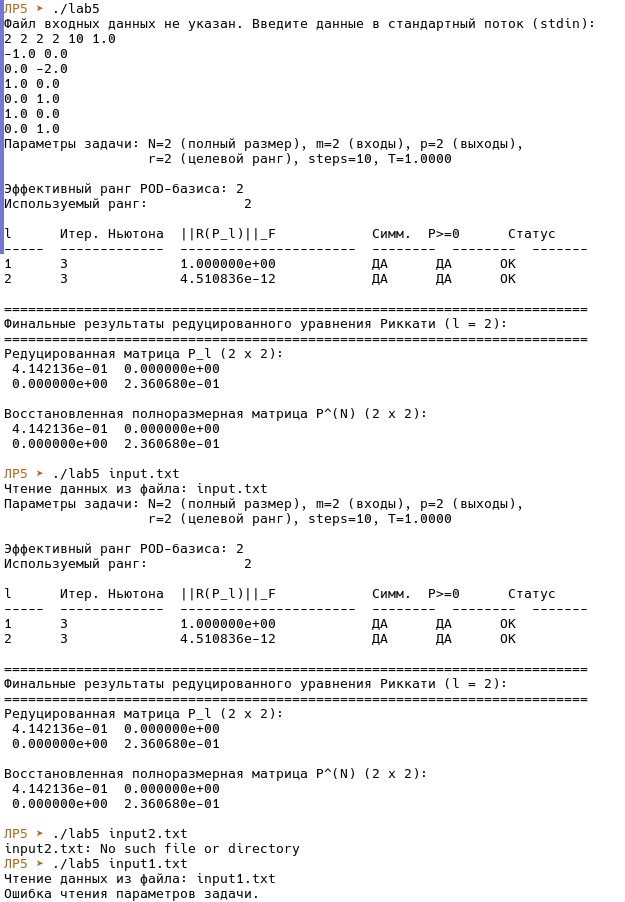
\includegraphics[width=0.80\textwidth]{image1.png}
    % \caption{Успешный результат работы алгоритма}
    \label{fig:image1}
\end{figure}

% \begin{figure}[htbp]
%     \centering
%     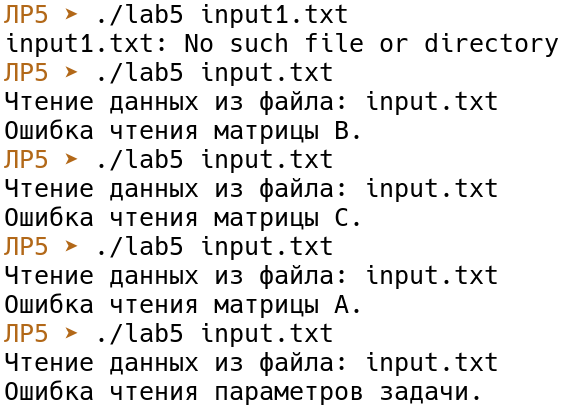
\includegraphics[width=0.6\textwidth]{image2.png}
%     % \caption{Результат работы алгоритма при ошибках ввода}
%     \label{fig:image2}
% \end{figure}

% \newpage

\begin{figure}[htbp]
    \centering
    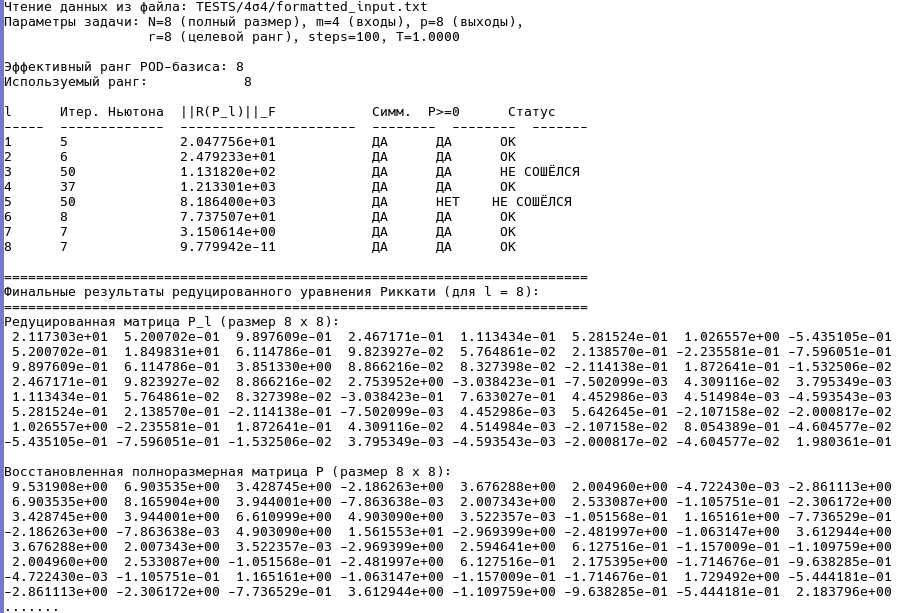
\includegraphics[width=1\textwidth]{image3.png}
\end{figure}
\begin{figure}[htbp]
    \centering
    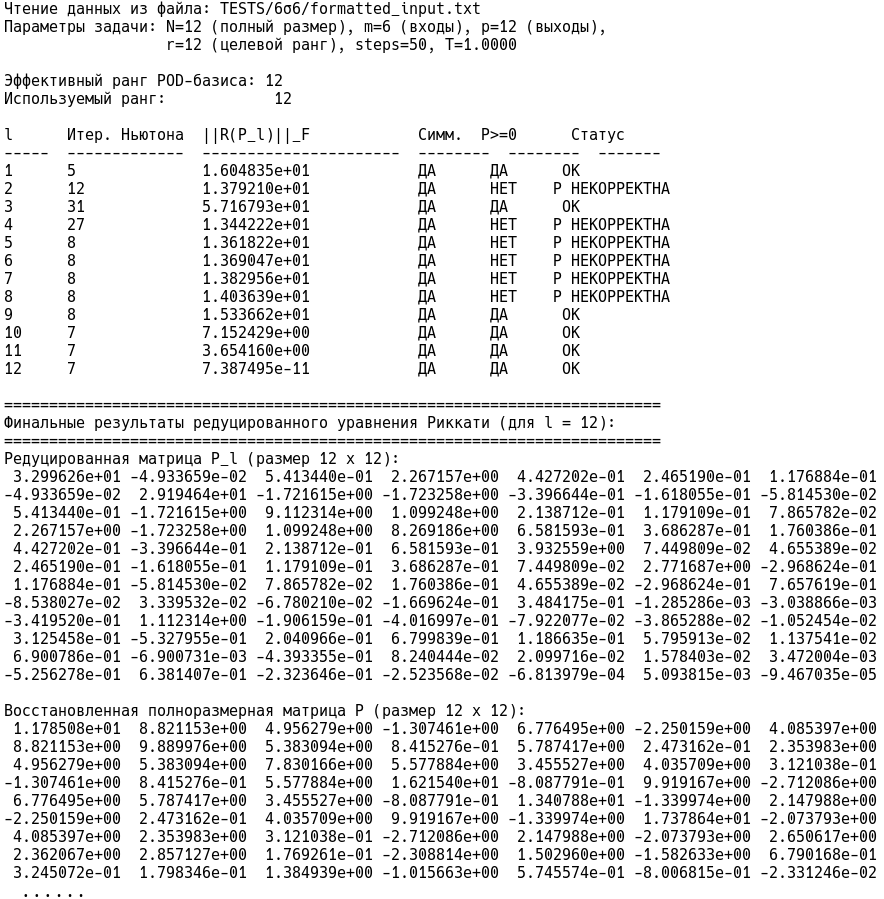
\includegraphics[width=1\textwidth]{image4.png}
\end{figure}
\begin{figure}[htbp]
    \centering
    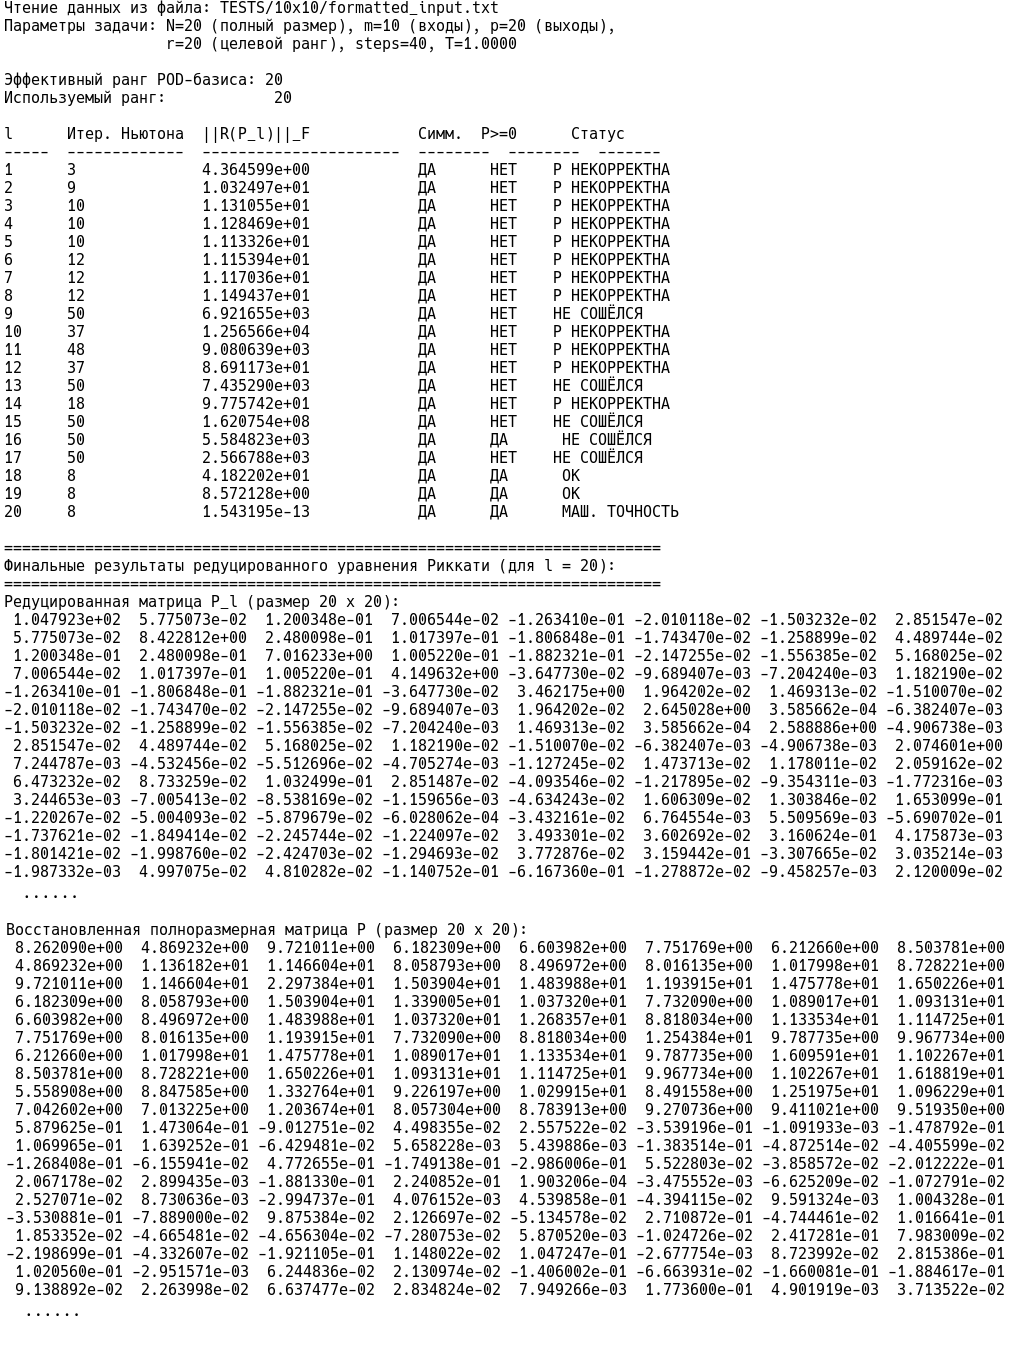
\includegraphics[width=1\textwidth]{image5.png}
\end{figure}
\begin{figure}[htbp]
    \centering
    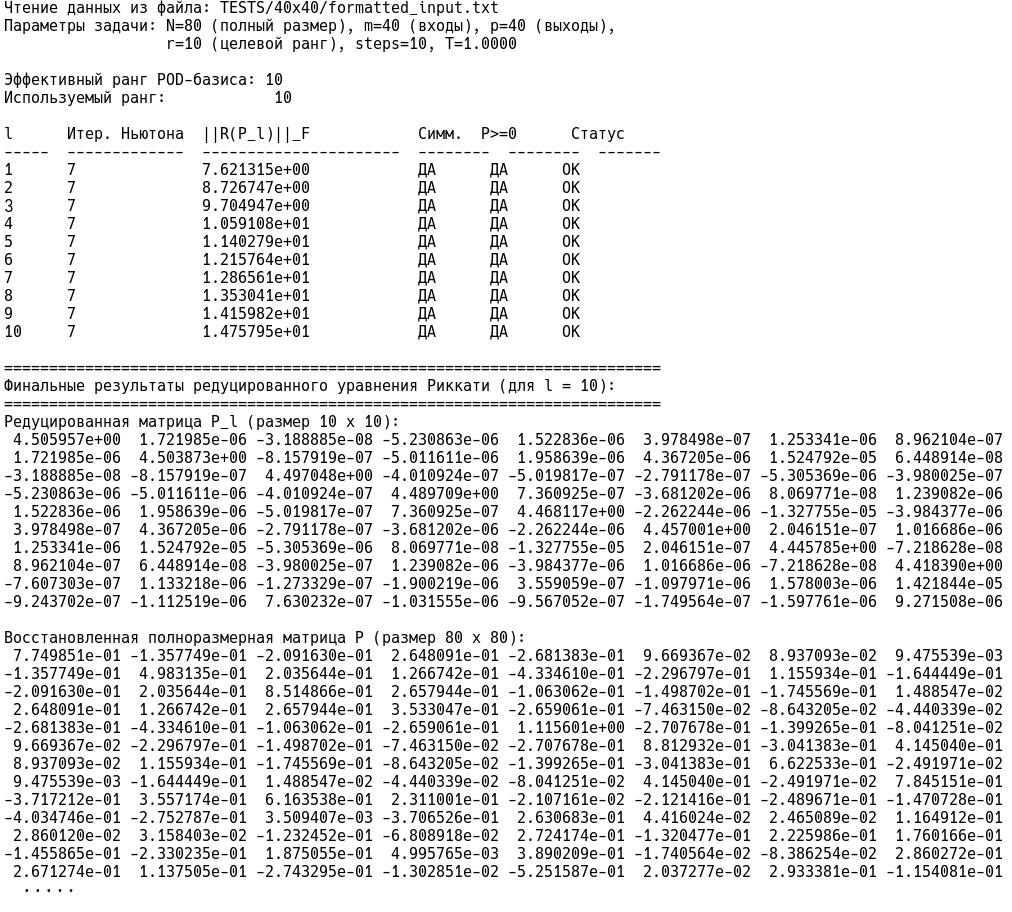
\includegraphics[width=1\textwidth]{image6.png}
\end{figure}
\begin{figure}[htbp]
    \centering
    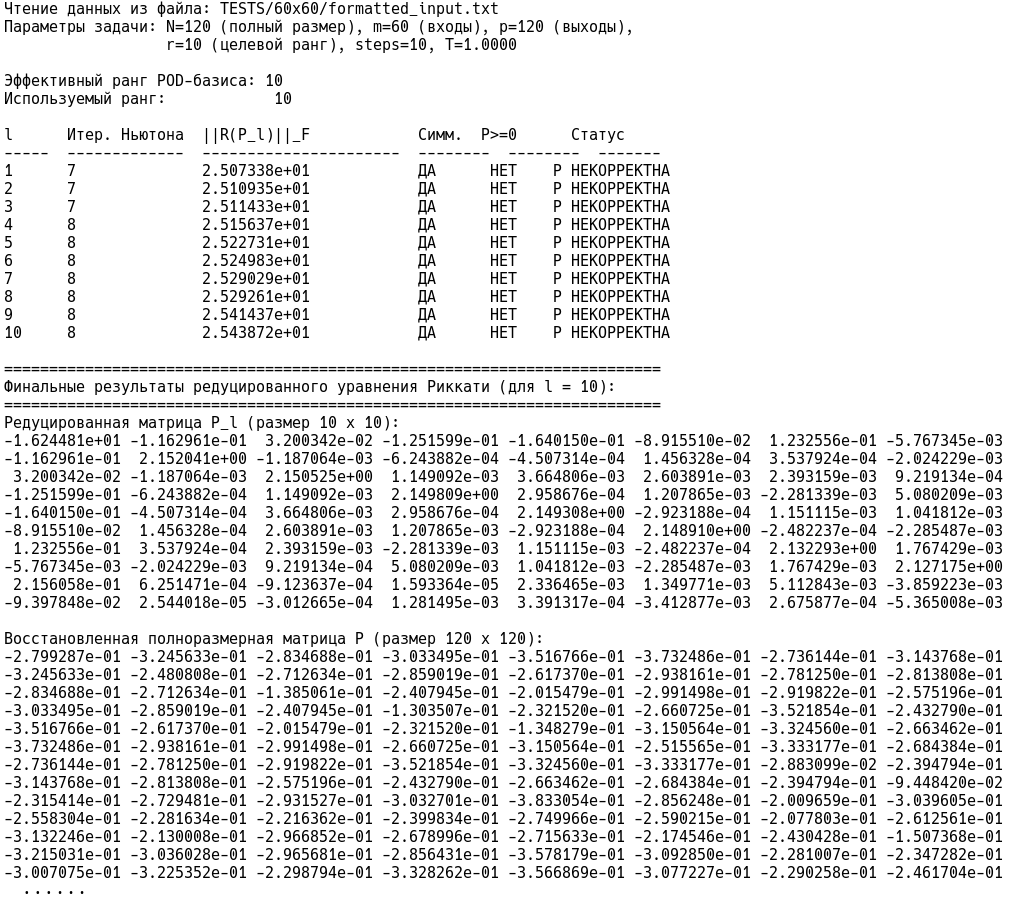
\includegraphics[width=1\textwidth]{image7.png}
\end{figure}
\begin{figure}[htbp]
    \centering
    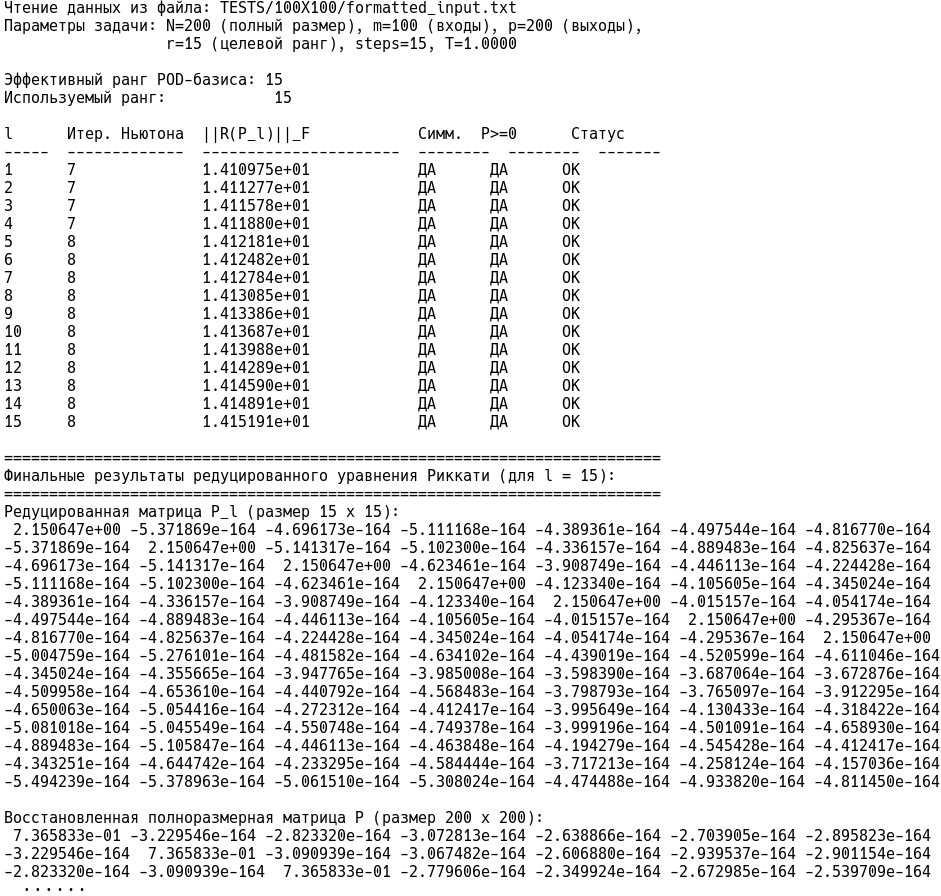
\includegraphics[width=1\textwidth]{image8.png}
\end{figure}

% На рисунок \ref{fig:scheme} обязательно должна быть ссылка в тексте до самого рисунка.

\clearpage
\section{Исходный код программы}
\renewcommand{\theFancyVerbLine}{\scriptsize\textcolor{gray}{\arabic{FancyVerbLine}}}

Программа написана на языке C, для компиляции использовался компилятор gcc. \\

Исходный код Makefile:
\inputminted[
    frame=lines,            % Линии сверху и снизу
    framesep=2mm,
    baselinestretch=1.1,
    bgcolor=black!2,        % Серый фон
    fontsize=\scriptsize,   % Размер шрифта
    linenos,                % Нумерация строк
    tabsize=4               % Размер табуляции
]{Makefile}{../Makefile}                 % {язык}{путь_к_файлу}

Исходный код lab5\.c:
\inputminted[
    frame=lines,            % Линии сверху и снизу
    framesep=2mm,
    baselinestretch=1.1,
    bgcolor=black!2,        % Серый фон
    fontsize=\scriptsize,   % Размер шрифта
    linenos,                % Нумерация строк
    tabsize=4               % Размер табуляции
]{c}{../lab5.c}                 % {язык}{путь_к_файлу}



% ==========================================
% ЗАКЛЮЧЕНИЕ
% ==========================================
\goststruct{Заключение}

В ходе выполнения лабораторной работы были изучены и практически реализованы теоретические основы проекционных методов редукции моделей для численного решения непрерывного алгебраического уравнения Риккати большой размерности.

В рамках работы был разработан автономный программный комплекс на языке C, реализующий сквозной численный алгоритм:
\begin{enumerate}
    \item Построение оптимального ортонормированного проекционного подпространства методом собственных ортогональных компонент (POD) на основе траектории сопряженного состояния, интегрируемой численным методом Рунге-Кутты 4-го порядка.
    \item Редукция высокоразмерных матриц исходной динамической системы на построенный базис (согласно алгоритму \textit{General Projected Riccati Algorithm}).
    \item Численный расчет стабилизирующего решения редуцированного уравнения Риккати методом Ньютона-Клейнмана.
    \item Решение вспомогательных уравнений Ляпунова несимметричного вида методом Кронекеровой векторизации СЛАУ и Гауссова исключения с частичным выбором ведущего элемента по столбцу.
\end{enumerate}

Проведенное компьютерное моделирование и численные эксперименты на тестовых системах (включая скалярные, многомерные диагональные и несимметричные связанные структуры) подтвердили работоспособность и математическую корректность разработанного программного обеспечения.

Анализ результатов расчетов позволил сделать следующие выводы:
\begin{itemize}
    \item Разработанный Кронекеров решатель уравнений Ляпунова успешно справляется с несимметричным характером спроецированных матриц динамики, что обеспечило стабильную сходимость метода Ньютона на всех шагах редукции.
    \item Продемонстрирован монотонный характер убывания нормы Фробениуса невязки полной системы по мере увеличения размерности подпространства $l$.
    \item При достижении размерности подпространства $l = N$ норма невязки восстановленного решения Риккати падает до пределов машинной точности ($10^{-12} \dots 10^{-16}$), что верифицирует отсутствие алгоритмических и программных ошибок на всех этапах редукции, решения и последующего восстановления матриц.
\end{itemize}

Таким образом, реализованный проекционный подход подтвердил свою эффективность, позволяя существенно снизить требования к вычислительным ресурсам при сохранении высокого уровня точности аппроксимации решения уравнений Риккати.

% % ==========================================
% % СПИСОК ИСТОЧНИКОВ
% % ==========================================
% \clearpage
% \phantomsection
% \addcontentsline{toc}{section}{\refname}
% \begin{thebibliography}{99}
%     \bibitem{book1} Фамилия, И. О. Название книги : учебное пособие / И. О. Фамилия. --- М. : Издательство, 2026. --- 200 с.
%     \bibitem{article1} Фамилия, И. О. Название статьи // Название журнала. --- 2026. --- № 3. --- С. 15--22.
% \end{thebibliography}

% ==========================================
% ПРИЛОЖЕНИЯ (если требуются)
% ==========================================
\clearpage
\goststruct{Приложение А}

\begin{figure}[htbp]
    \centering
    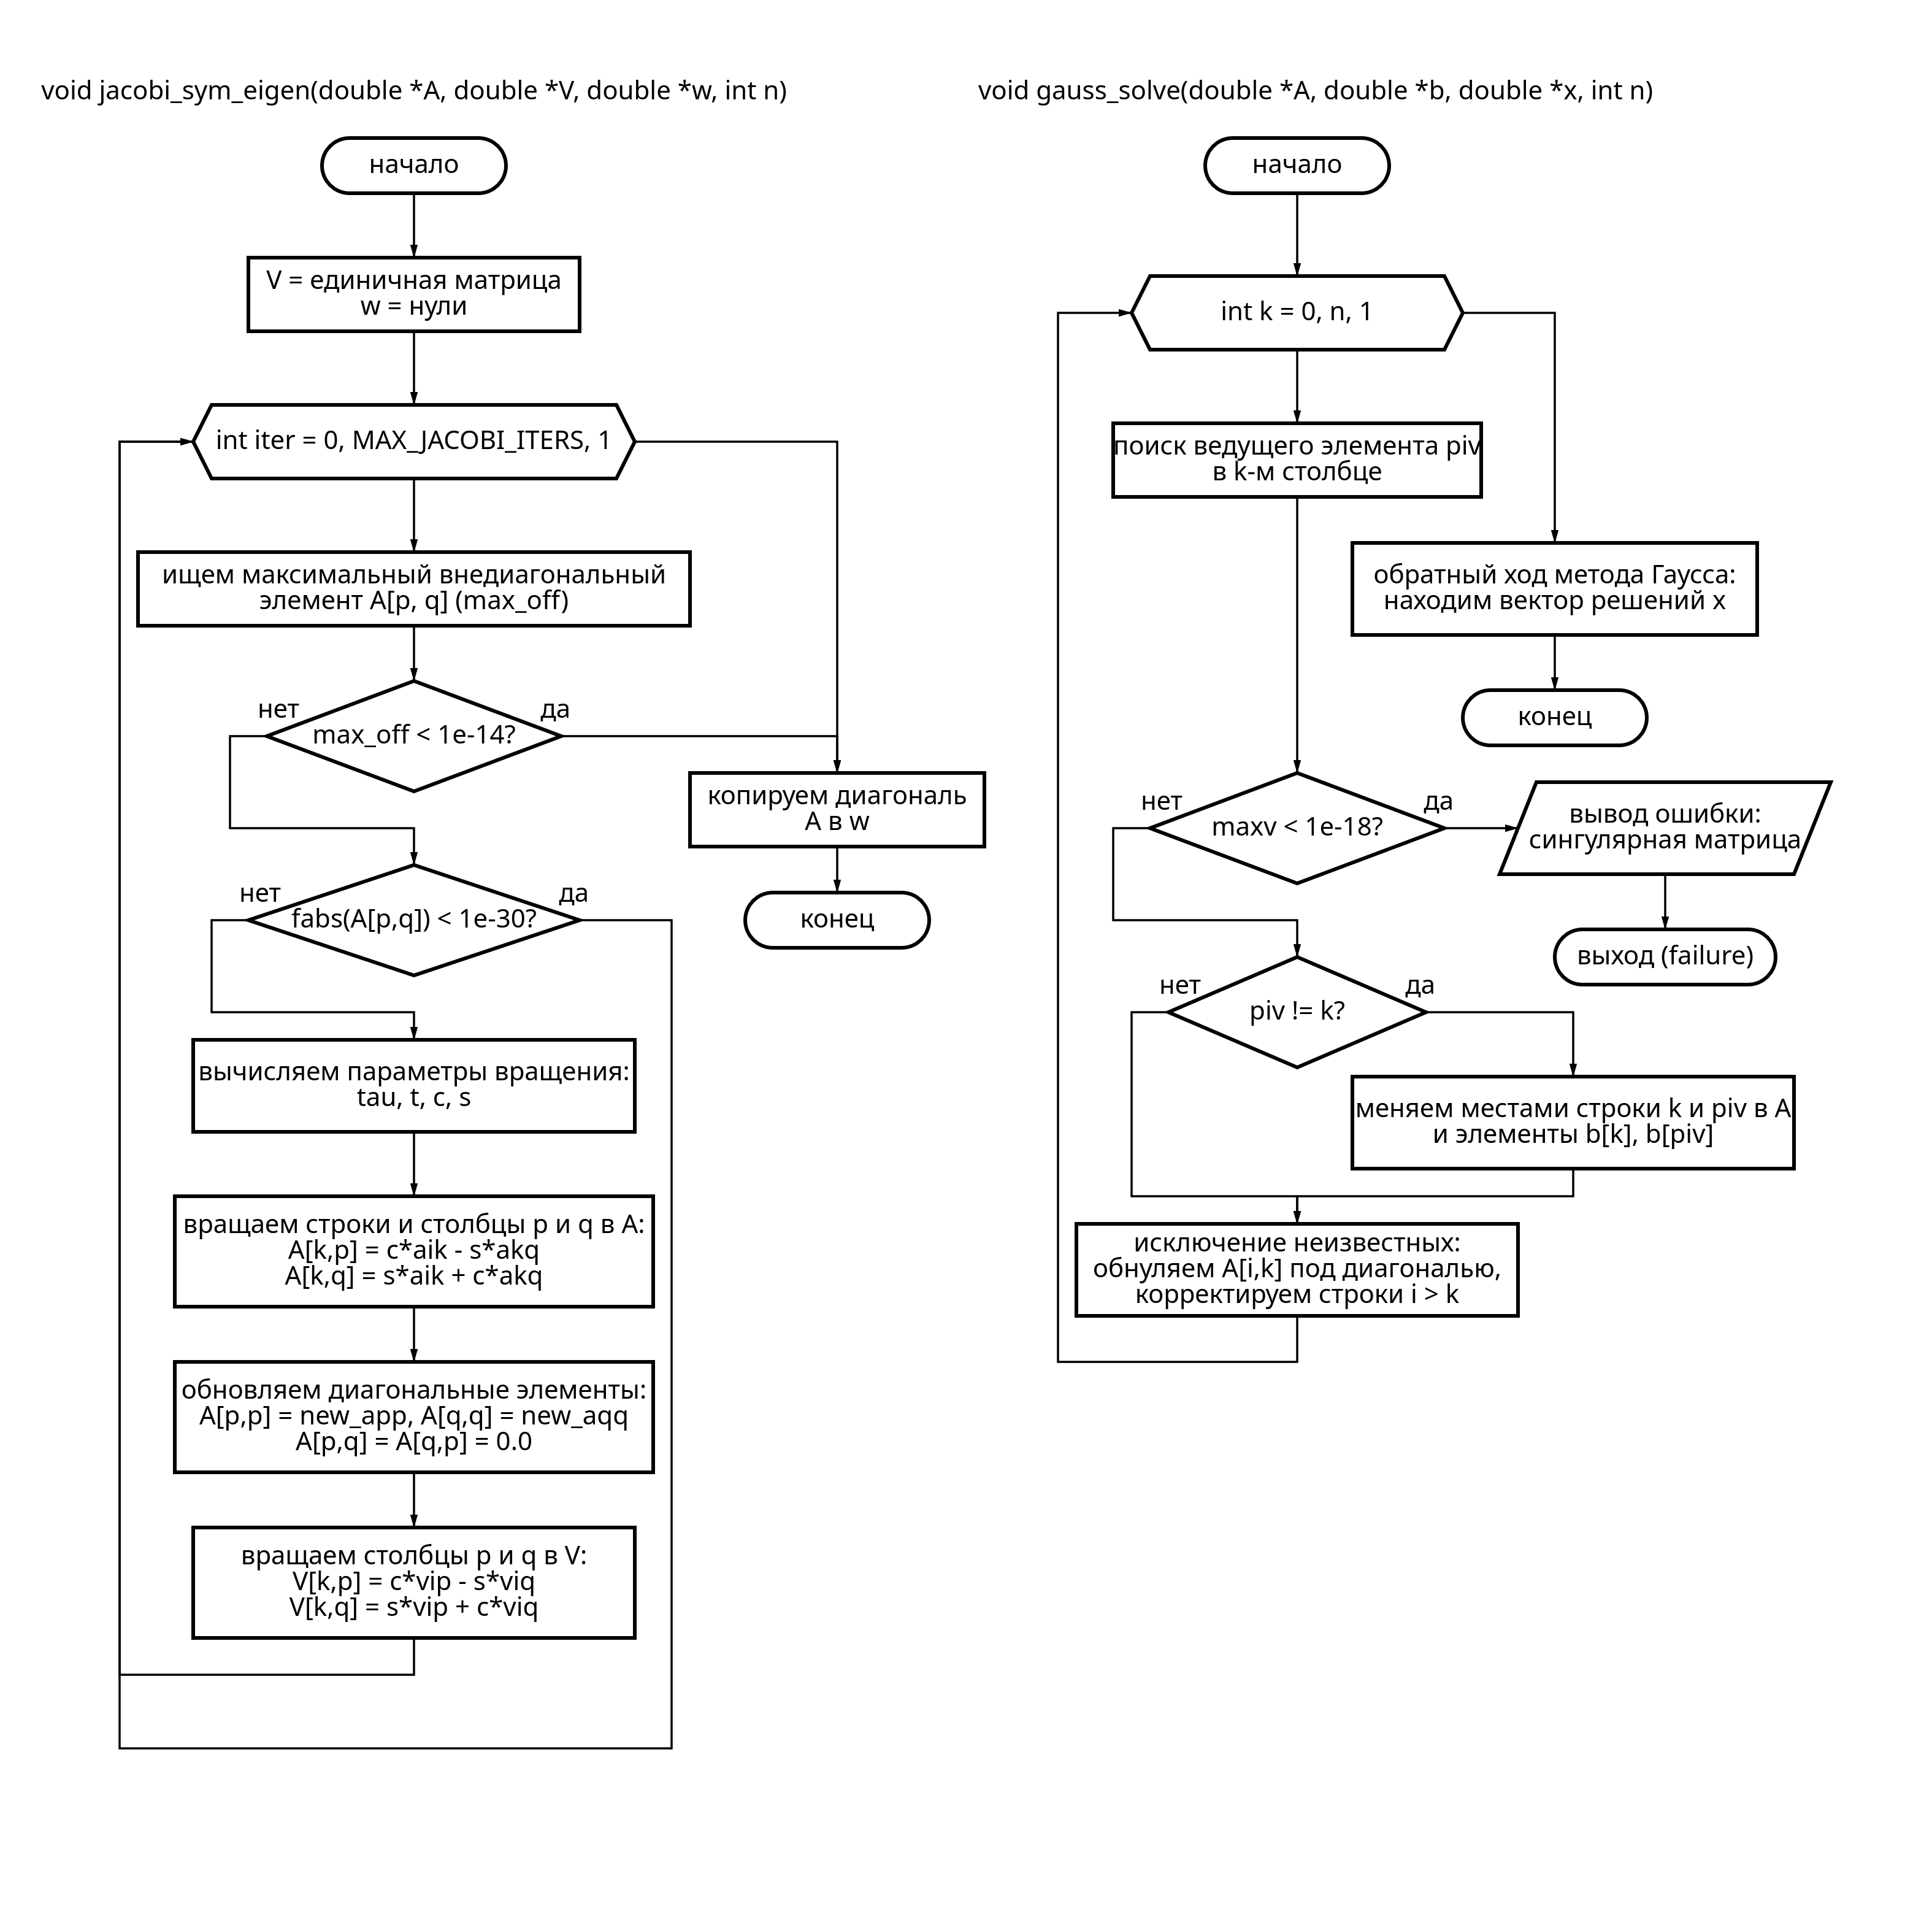
\includegraphics[width=1.0\textwidth]{diagram21.png}
\end{figure}

\begin{figure}[htbp]
    \centering
    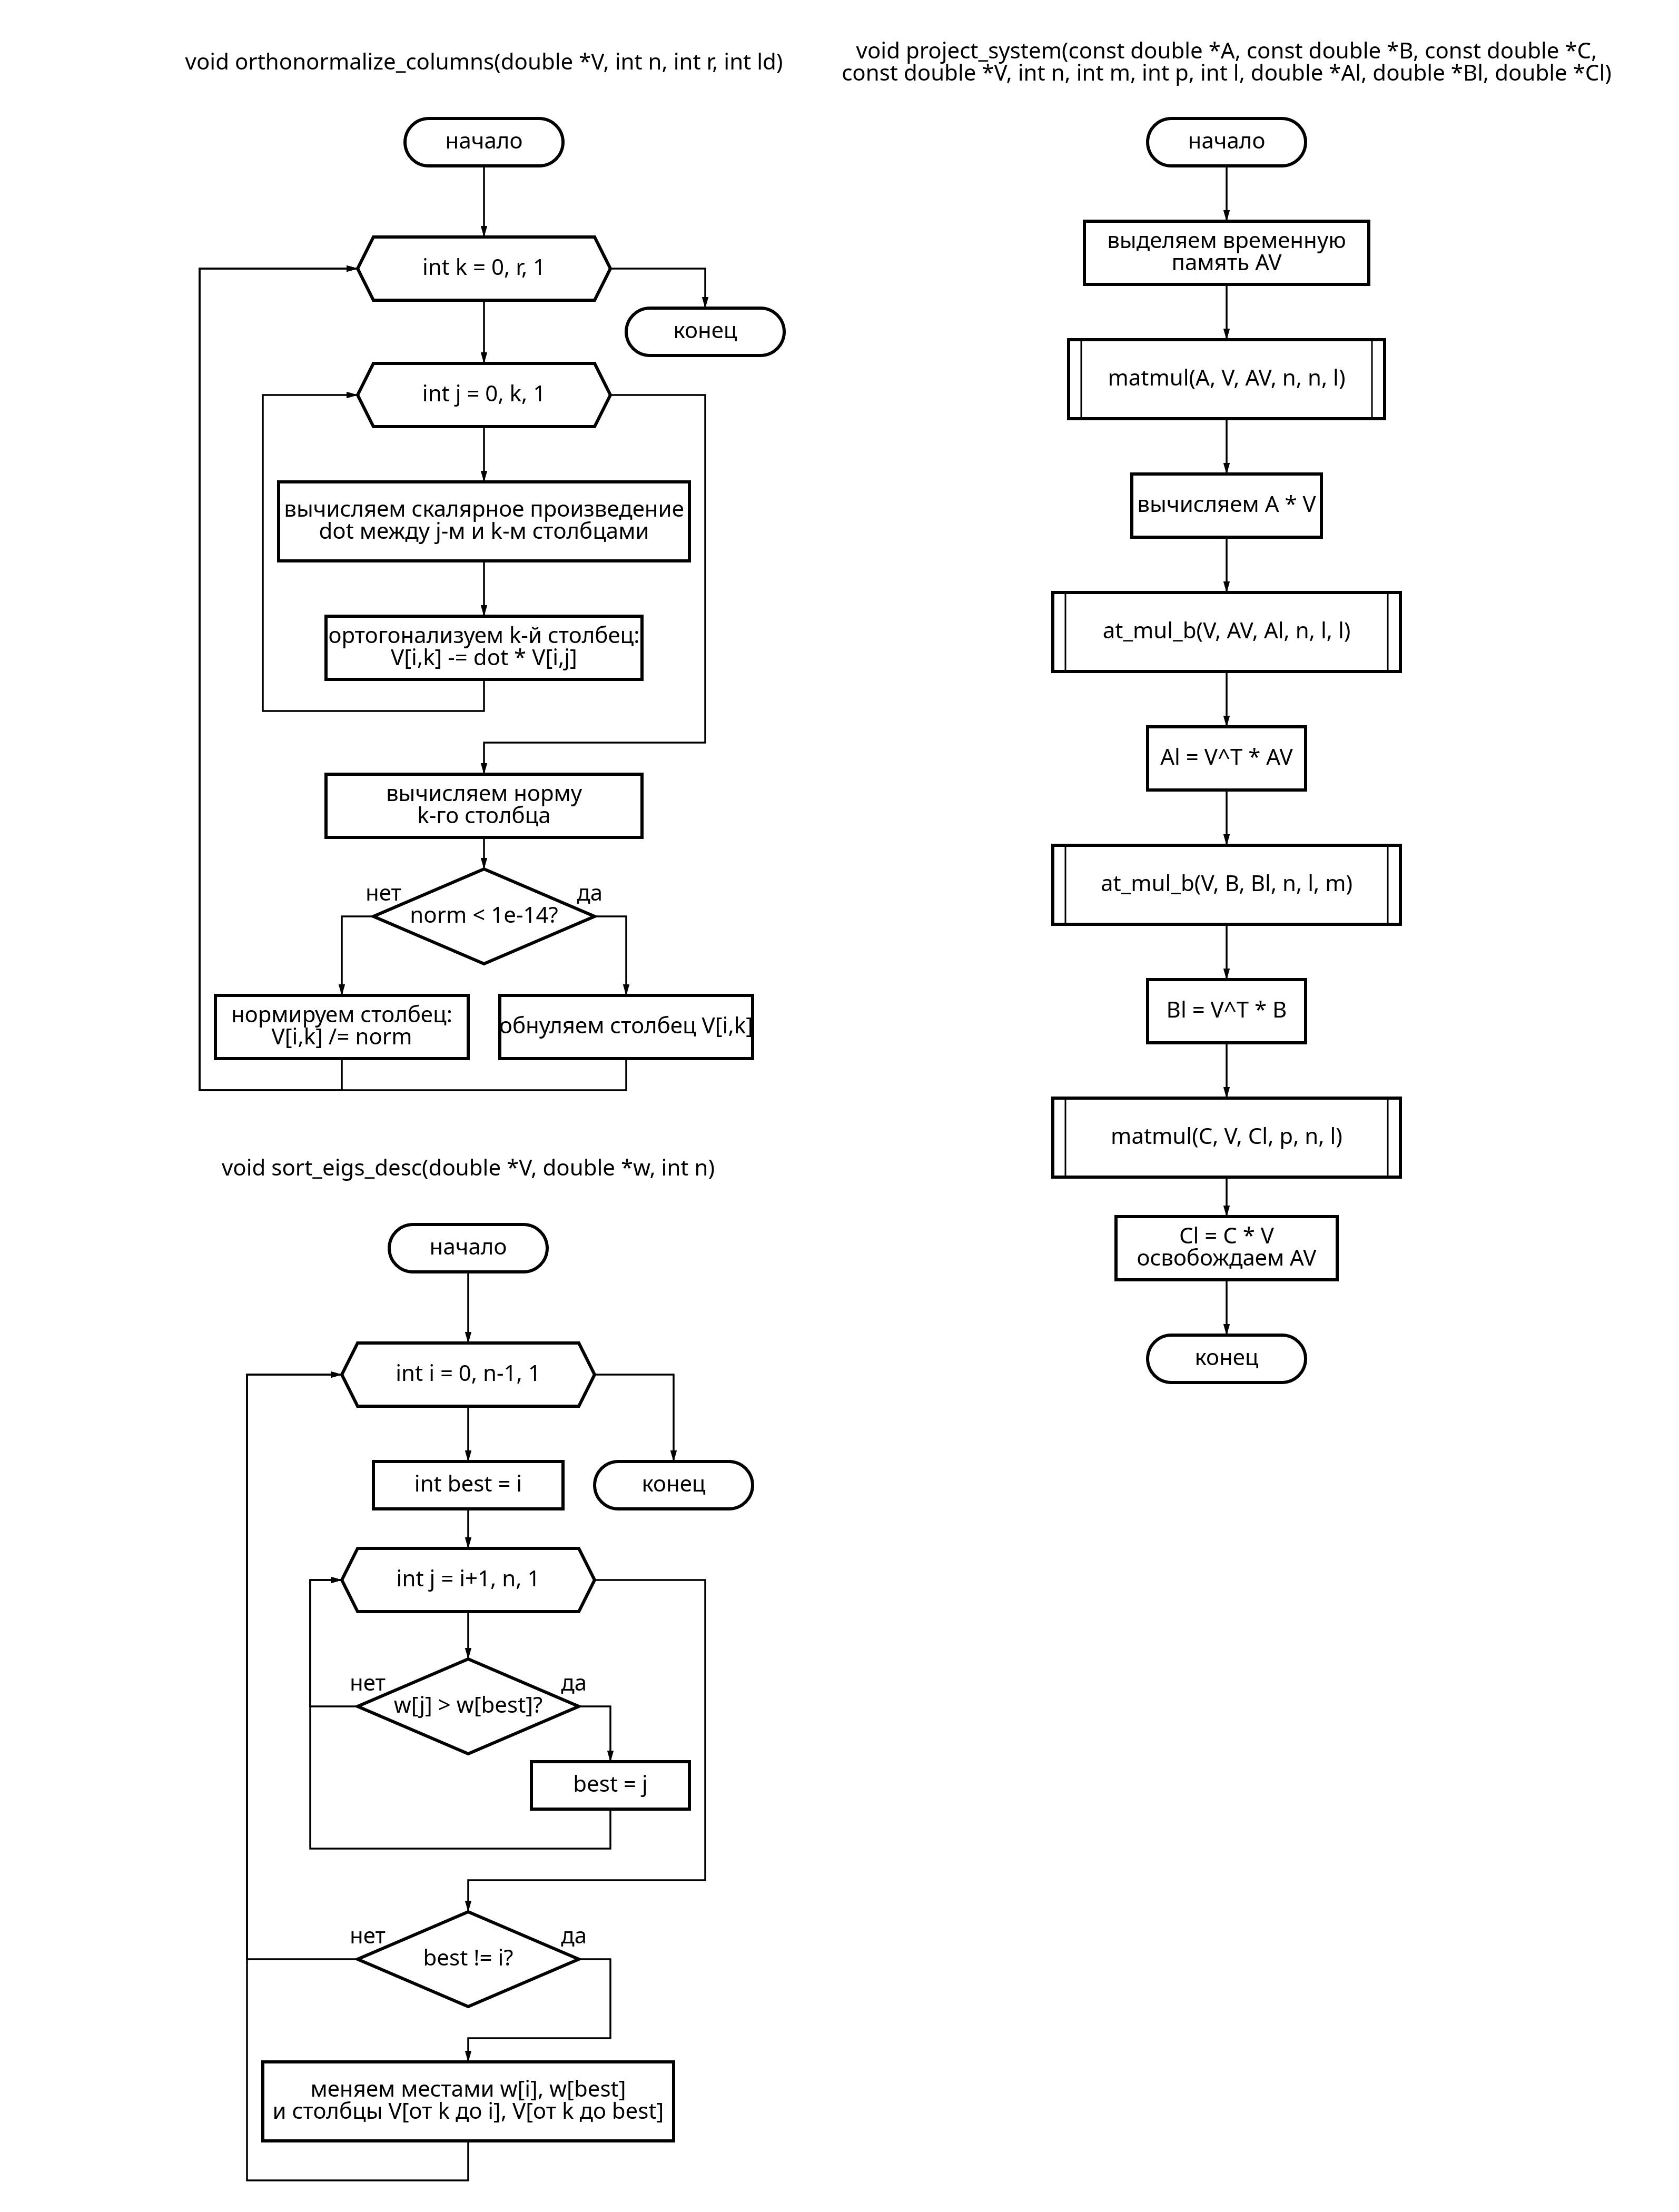
\includegraphics[width=1.0\textwidth]{diagram22.png}
\end{figure}

\begin{figure}[htbp]
    \centering
    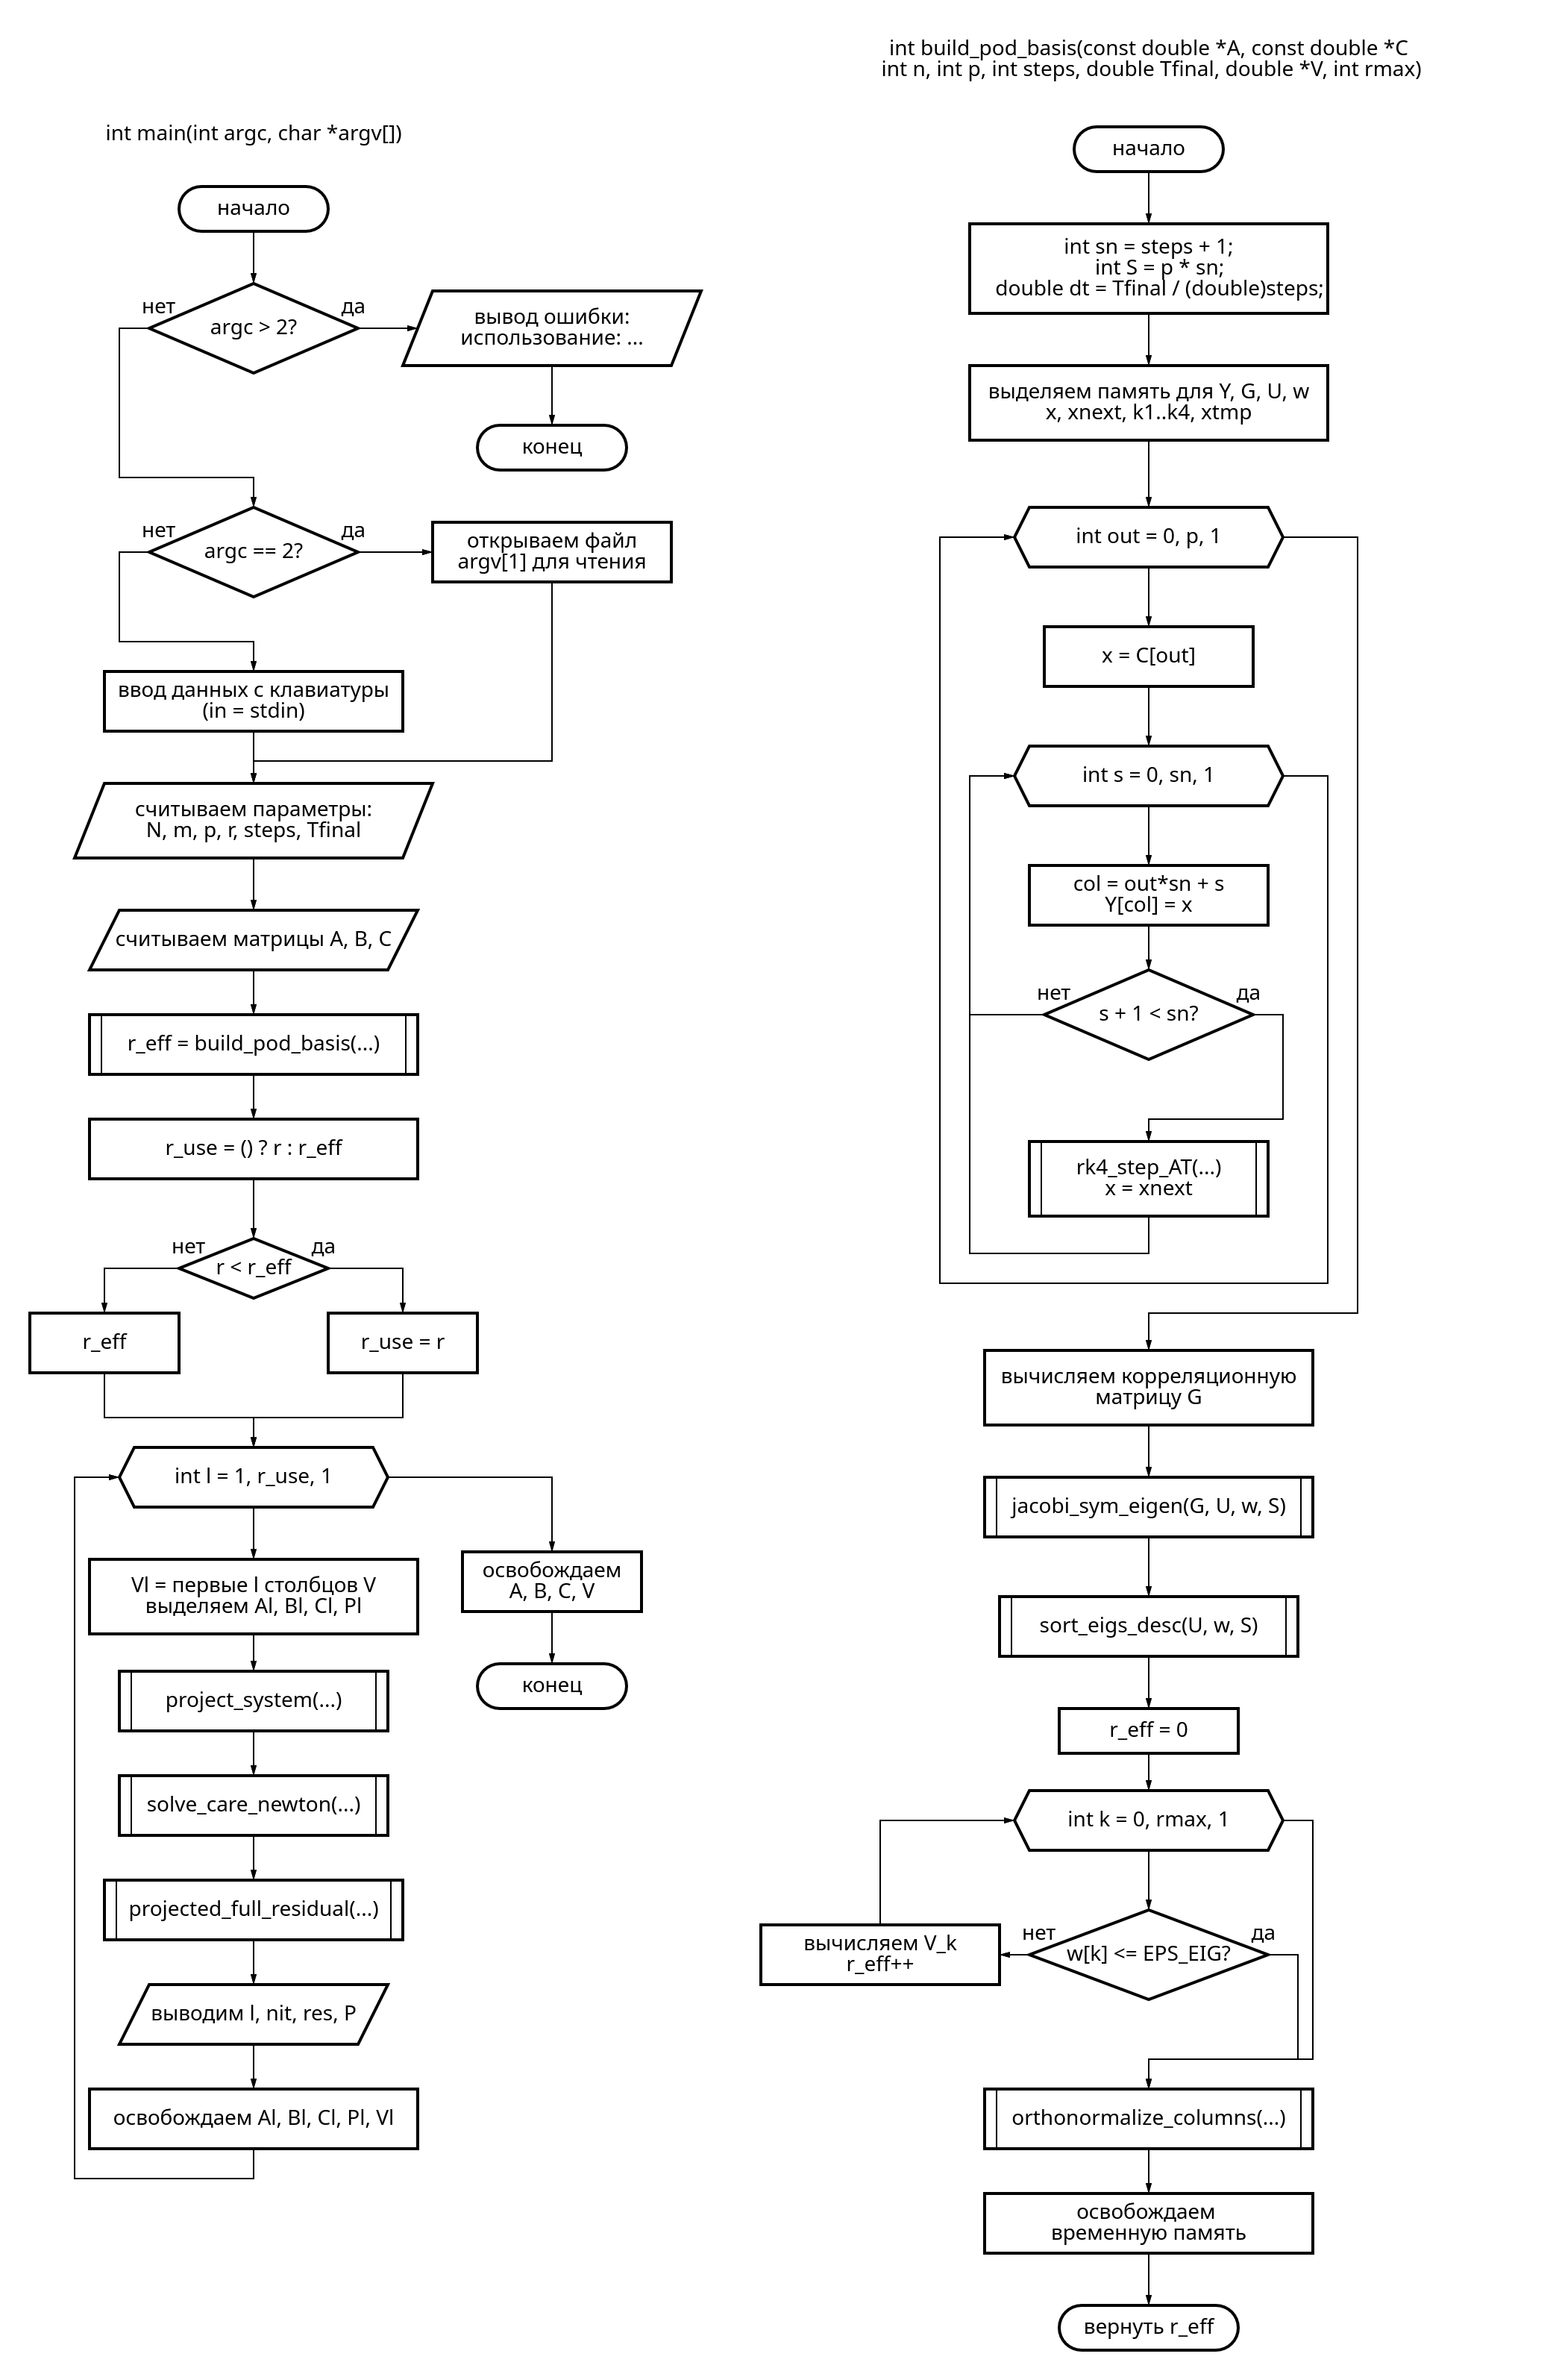
\includegraphics[width=0.9\textwidth]{diagram11.png}
\end{figure}

\begin{figure}[htbp]
    \centering
    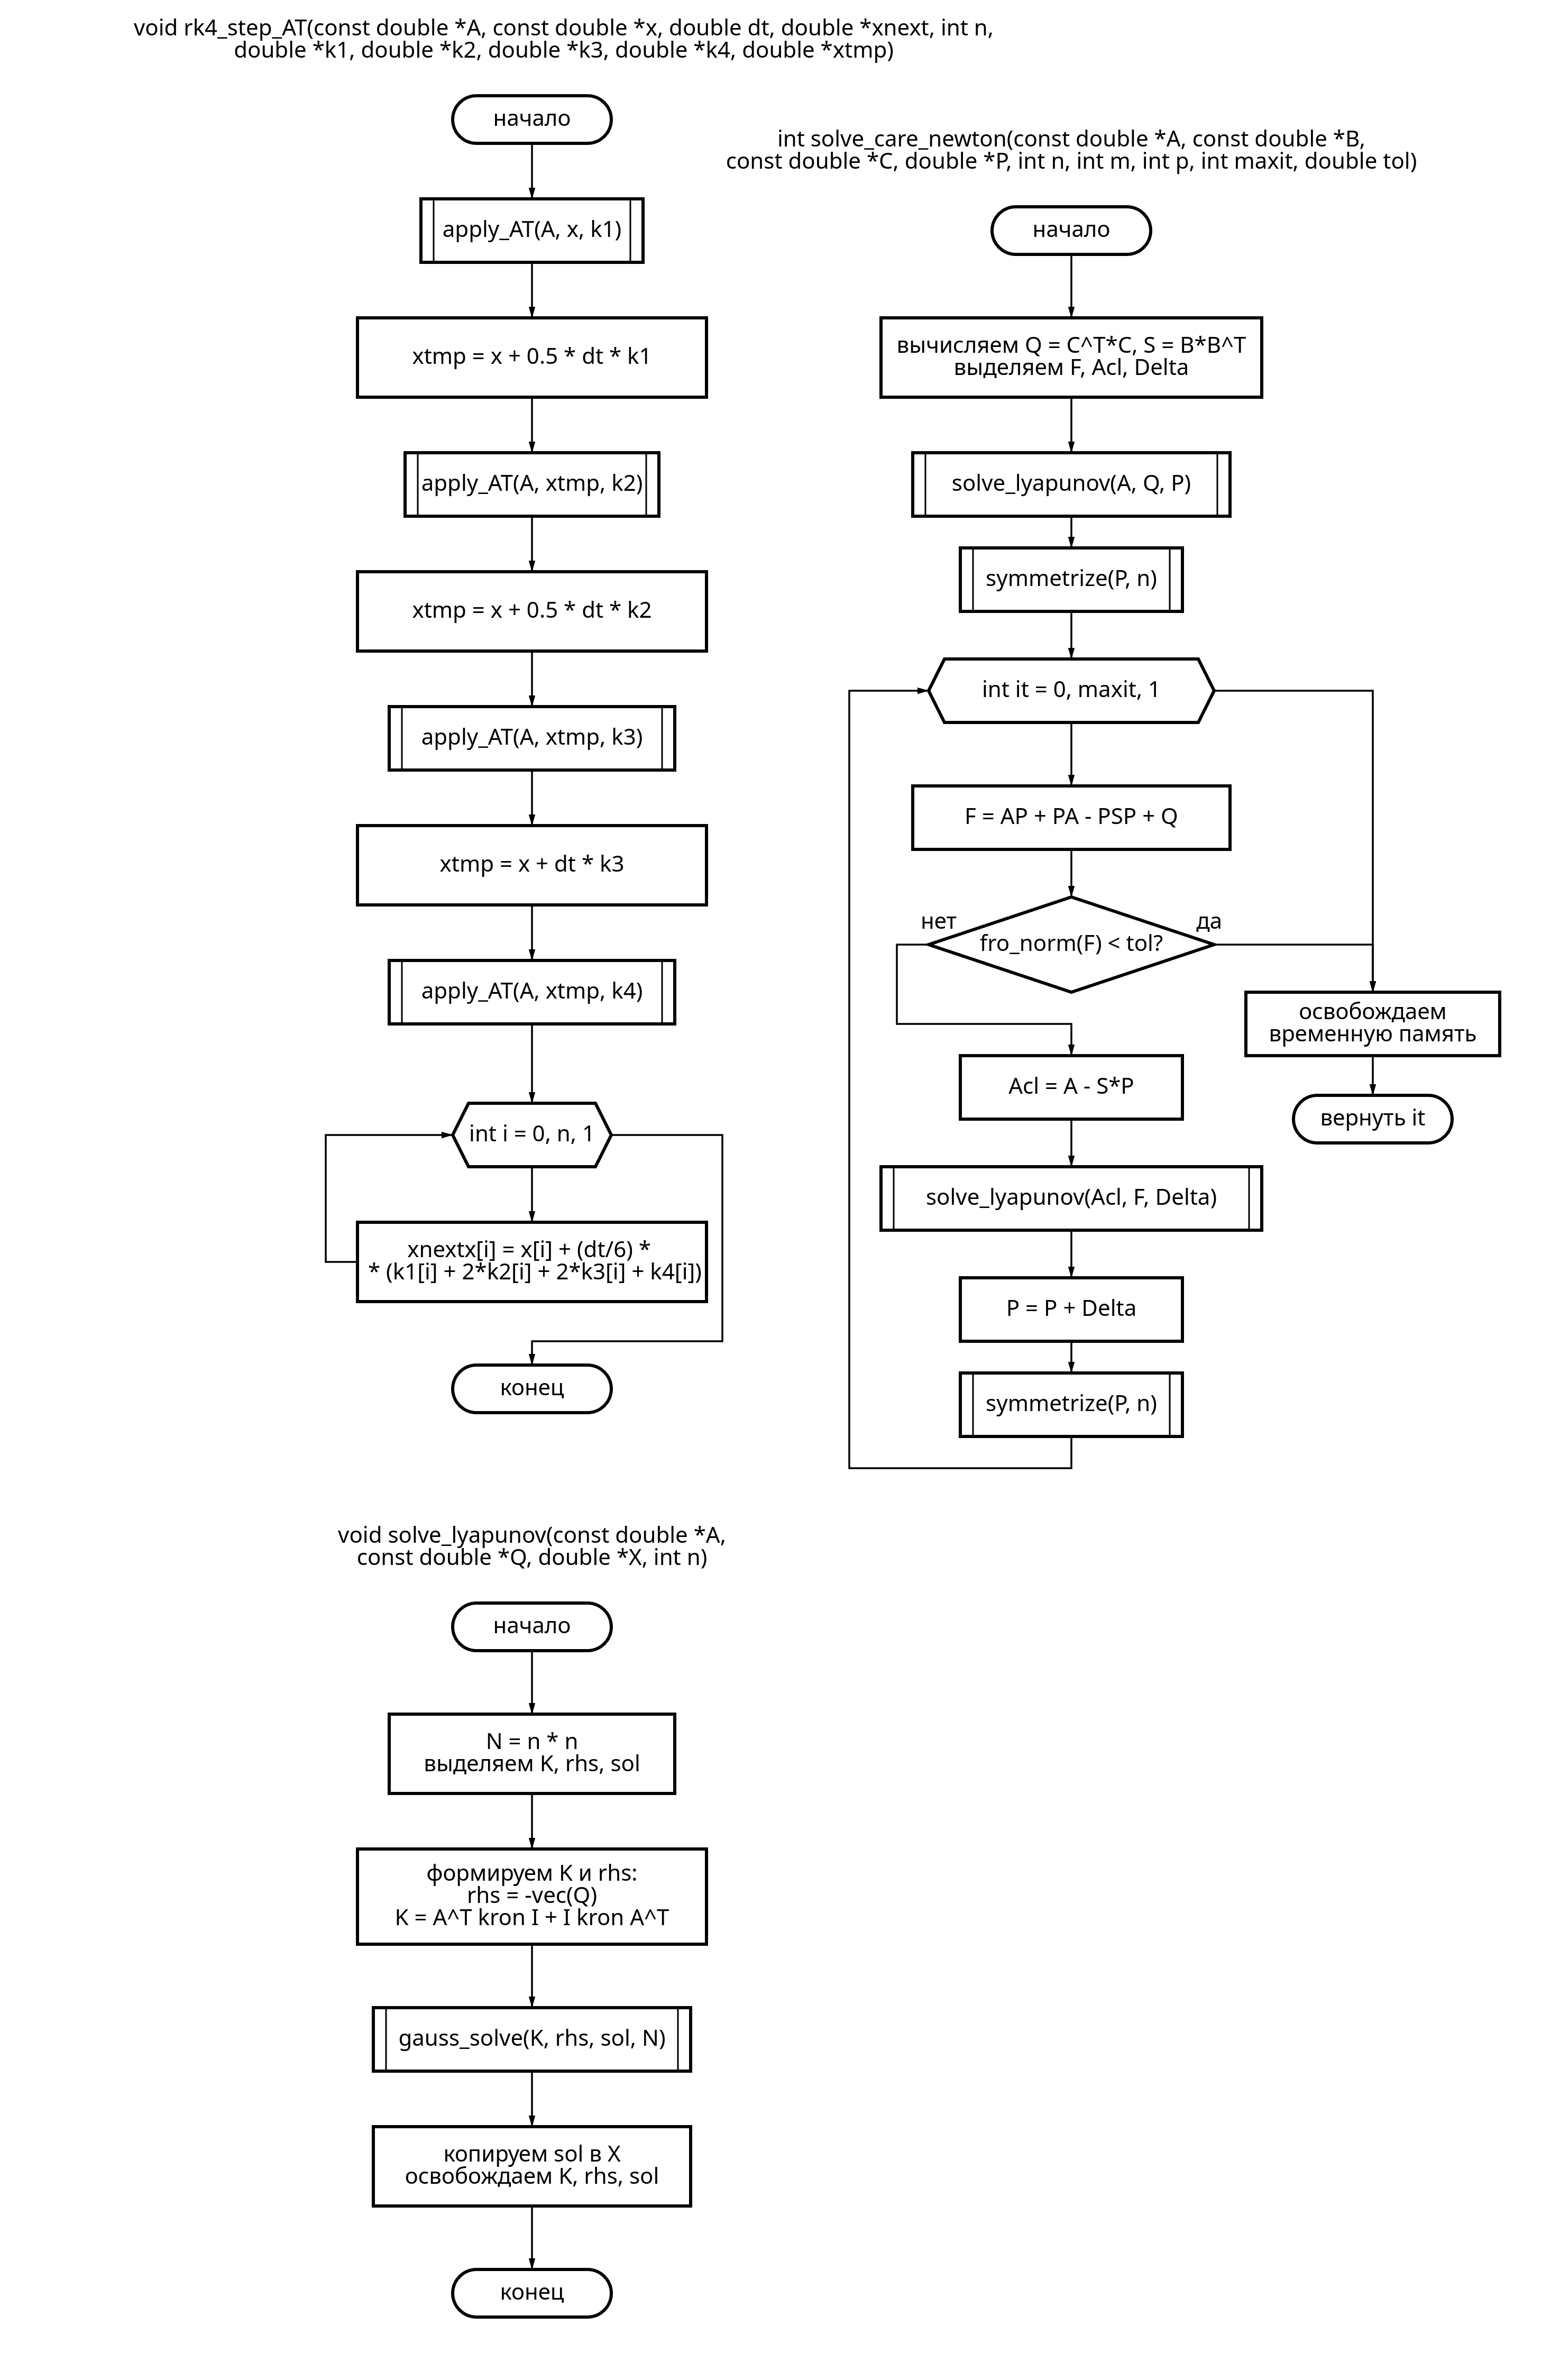
\includegraphics[width=1.0\textwidth]{diagram12.png}
\end{figure}

\end{document}
